\documentclass[12pt,a4paper]{report}
\usepackage{url}
\usepackage{graphics}
\usepackage{textcomp}
\usepackage[official]{eurosym}
\usepackage{amsmath}
\usepackage{amssymb}
\usepackage{amsthm}
\usepackage[pdftex]{graphicx}
\usepackage{sidecap}
\usepackage{subfigure}
\usepackage{verbatim}
\usepackage[small]{caption}
\usepackage{rotating}
\usepackage{listings}
\usepackage{fancyvrb}
\VerbatimFootnotes
\usepackage{color}
\usepackage[toc,page]{appendix}
\usepackage{lscape}
\usepackage{placeins}
\usepackage[all]{xy}
\usepackage{wrapfig}
\usepackage{multicol}
\usepackage{multirow}
\usepackage{enumerate}
\usepackage{setspace}
% Below are the spacing options.
%\doublespacing
%\singlespacing
\onehalfspacing
%\setstretch{1.8}

\newtheorem*{definition}{Definition}
\newtheorem*{example}{Example}
\newtheorem*{theorem}{Theorem}
\newtheorem*{theorem*}{Theorem}
\newcommand{\pde}{partial differential equation}
\newcommand{\Pde}{Partial differential equation}
\newcommand{\pdes}{partial differential equations}
\newcommand{\Pdes}{Partial differential equations}

% This is the standardone inch all around border.
%\usepackage{fullpage}

% This is what I've made myself - max space used, for Tisseur cw.
% For most stand alone work, use this one.
%\setlength{\topmargin}{-1in}
%\setlength{\textheight}{9.75in}
%\setlength{\oddsidemargin}{-0.25in}
%\setlength{\textwidth}{7in}

% This is the geometry package... apparently good!
%\usepackage[left=2cm,top=4cm,right=2cm]{geometry}
\usepackage[a4paper]{geometry}
\geometry{top=1.0in, bottom=1.0in, left=1.6in, right=1.0in}

\lstset{numbers=left, stepnumber=2, frame=single,basicstyle=\footnotesize, showstringspaces=false, language=C++}



\begin{document}
%\begin{titlepage}
\begin{center}
\vspace*{1in}
{\Huge MODIFICATION OF THE \vspace*{0.3in} PARALLEL \vspace*{0.3in} PRECONDITIONERS FOR THE INCOMPRESSIBLE \vspace*{0.3in} NAVIER-STOKES EQUATIONS}

\vspace*{1.5in}

{A THESIS SUBMITTED TO THE UNIVERSITY OF MANCHESTER \\ FOR THE
DEGREE OF MASTER OF SCIENCE \\ IN THE FACULTY OF ENGINEERING AND PHYSICAL SCIENCES}

\vspace*{1.5in}

{2010}

\vspace*{1.5in}

{{\bfseries Raymon White} \\ School of Computer Science}

\end{center}

\end{titlepage}

%\thispagestyle{empty}

\pagestyle{plain}
\pagenumbering{arabic}
\setcounter{page}{1}

%\tableofcontents
%\listoffigures
%\listoftables

%\chapter*{ABSTRACT}
%\addcontentsline{toc}{chapter}{ABSTRACT}
%  \begin{center}
    Modification of the parallel preconditoners for the incompressible Navier-Stokes equations \\
    Authors: Raymon White
  \end{center}
[Insert abstract]
  \begin{center}
    Supervisors: Milan Mihajlovic and Matthias Heil.
  \end{center}


%\chapter*{DECLARATION}
%\addcontentsline{toc}{chapter}{DECLARATION}
%No portion of the work referred to in the thesis has been
submitted in support of an application for another degree or
qualification of this or any other university or other institute of
learning



%\chapter*{COPYRIGHT STATEMENT}
%\addcontentsline{toc}{chapter}{COPYRIGHT STATEMENT}
%\begin{enumerate}[i.]
  \item The author of this thesis (including any appendices and/or schedules to this thesis) owns certain copyright or related rights in it (the  “Copyright”)and s/he has given The University of Manchester certain rights to use such Copyright, including for administrative purposes.
  \item Copies of this thesis, either in full or in extracts and whether in hard or electronic copy, may be made \textbf{only} in accordance with the Copyright, Designs and Patents Act 1988 (as amended) and regulations issued under it or, where appropriate, in accordance with licensing agreements which the University has from time to time. This page must form part of any such copies made.
  \item The ownership of certain Copyright, patents, designs, trade marks and other
intellectual property (the “Intellectual Property”) and any reproductions of copyright works in the thesis, for example graphs and tables (“Reproductions”), which may be described in this thesis, may not be owned by the author and may be owned by third parties. Such Intellectual Property and Reproductions cannot and must not be made available for use without the prior written permission of the owner(s) of the relevant Intellectual Property and/or Reproductions.
  \item Further information on the conditions under which disclosure, publication and commercialisation of this thesis, the Copyright and any Intellectual Property and/or Reproductions described in it may take place is available in the University IP Policy (see \url{http://www.campus.manchester.ac.uk/medialibrary/policies/intellectual-property.pdf}), in any relevant \newline Thesis restriction declarations deposited in the University Library, The University    Library’s regulations (see \url{http://www.manchester.ac.uk/library/aboutus/regulations}) and in The University’s policy on presentation of Theses.
\end{enumerate}


%\chapter*{ACKNOWLEDGEMENT}
%\addcontentsline{toc}{chapter}{ACKNOWLEDGEMENT}
%\begin{quotation}
I would like to thank Matthias Heil and Milan Mihajlovic, for their supervision, advice and guidance throughout the duration of my dissertation. [More to add here.]
\end{quotation}


\chapter{A review of OOMPH-LIB's Block Preconditioning Framework\label{chap:block_preconditioning_framework}}
In this document we review the features of \texttt{oomph-lib}'s block 
preconditioning framework. We describe the functionality of the 
framework starting from the implementation of a simple block diagonal 
preconditioner. Then we introduce the LSC (Least Square Commutator) 
preconditioner for the Navier-Stokes equations~\cite{fastiterativesolvers}. 
Finally, we discuss the implementation of the augmented Lagrangian 
preconditioner for the solution of the constrained Navier-Stokes equations with
Lagrange multipliers.

the purpose of the block preconditioning framework (BPF) is to facilitate 
efficient implementation of the block preconditioners in a distributed 
environment. As such, it represents a software middleware which enables 
sytematic hierachical construction of block preconditioners for arbitrarily 
complex multiphysics problems by reusing the existing efficient preconditioners
for the constituent single physics sub-problems. At the same time the BPF hides
from the end user tedious implementation details associated with blocking of 
the Jacobian and the distribution of these blocks among the processors (these 
procedures involve the intricate communication with other parts of the library 
to obtain the necessary information). The operations performed by the BPF add 
only a minor computational overhead to the total solution time thus retaining 
asymptotically the same performance as the constituent scalar problem solvers 
(such as AMG). (CITE RICHARD THESIS AND PAGE NUMBER)

\section{ Theoretical Background\label{sec:theoretical_background}}
In \texttt{oomph-lib}, all problems are solved by Newton's method, which requires
the (if the problem is not linear, repeated) solution of linear systems of the 
form

\begin{equation}
J\;\mathbf{\delta x} = -\mathbf{r}
\label{eq:linear_system1}
\end{equation}
for the Newton correction $\mathbf{\delta x}$ where $J$ is the
Jacobian matrix and $\mathbf{r}$ is the vector of non-linear residuals. (Left) 
preconditioning represents a transformation of the original linear system 
\eqref{eq:linear_system1} to
\begin{equation*}
P^{-1}J\;\mathbf{ \delta x}=-P^{-1}\mathbf{r}
\end{equation*}
is introduced with the aim of accelerating the convergence of Krylov subspace 
iterative methods such as GMRES or CG (CITE saad). The application of the 
preconditioner requires the solution of a linear system
\begin{equation*}
P\mathbf{z}=\mathbf{y}
\end{equation*}
for $\mathbf{z}$ at each Krylov iteration.

Block preconditioning requires special enumeration schemes for the unknowns 
(equivalent to reordering the linear systems) where all the unknowns 
corresponding to each type of DOF are grouped together and enumerated 
consecutively. This leads to a natural block structure of the linear systems.
This process is equivalent to the following transformation
\begin{equation*}
  \underbrace{P_{\pi} A P_{\sigma}}_{\tilde{A}} \underbrace{P_{\sigma}^{\mathsf{T}}\mathbf{x}}_{\tilde{\mathbf{x}}}=\underbrace{P_{\pi}\mathbf{f}}_{\tilde{\mathbf{f}}}
\end{equation*}
where $P_{\pi}$ and $P_{\sigma}$ are the permutation matrices.

For instance, linear elasticity problems[CITE] involve the solid (the nodal positions in the solid domain) degrees of freedom (DOFs). Consider the two-dimensional case, we begin by reordering the linear system to group together the two types of DOF 
\begin{equation*}
\begin{bmatrix}
 J_{xx} & J_{xy} \\
 J_{yx} & J_{yy}
\end{bmatrix}
\begin{bmatrix}
 \mathbf{\delta x_x} \\
 \mathbf{\delta x_y} 
\end{bmatrix}
=
\begin{bmatrix}
 \mathbf{r_x} \\
 \mathbf{r_y}
\end{bmatrix},
\end{equation*}
then the block diagonal preconditioner of the form 
\begin{equation*}
P_{diag}=
\begin{bmatrix}
J_{xx}&     \\
      &J_{yy}
\end{bmatrix}
\end{equation*}
is obtained by omitting the off-diagonal blocks from the Jacobian [CITE].
The application of the preconditioner requires the exact or approximate 
solution of the linear system
\begin{equation*}
\begin{bmatrix}
J_{xx}& \\
      &J_{yy}
\end{bmatrix}
\begin{bmatrix}
\mathbf{z_x}\\
\mathbf{z_y}
\end{bmatrix}
=
\begin{bmatrix}
\mathbf{y_x}\\
\mathbf{y_y}
\end{bmatrix},
\end{equation*}
the two sub-blocks will be solved directly. The vector $\mathbf{y}$ is the 
linear residual at the current GMRES iteration.

%%%%%%%%%%%%%%%%%%%%%%%%%%%%%%%%%%%%%%%%%%%%%%%%%%%%%
%%% FRAMEWORK OVERVIEW
%%%%%%%%%%%%%%%%%%%%%%%%%%%%%%%%%%%%%%%%%%%%%%%%%%%%%
\section{ Framework Overview\label{sec:framework_overview}}
The above example shows that the application of block preconditioners
require several generic steps:
\begin{itemize}
\item The classification of the DOFs.
\item The application of subsidiary preconditioning operators.
\end{itemize}
The following subsections describe how these tasks are performed
within \texttt{oomph-lib}'s block preconditioning framework.

%%%% BLOCK PRECONDITIONABLE ELEMENTS
\subsection{Block Preconditionable Elements\label{sec:block_preconditionable_elements}}
The DOFs need to be classified into different types so that the BPF knows how
to group the DOFs which it then assemble into sub-matrices for the 
preconditioner blocks. The classification of DOFs is implemented at an 
elemental level. The class \texttt{GeneralisedElement} contains two broken 
virtual functions that must be re-implemented to label the DOFs with their 
type. The functions are:
\begin{itemize}
\item \texttt{GeneralisedElement::ndof\_types()} must return the number of DOF 
types associated with an element.
\item \texttt{GeneralisedElement::get\_dof\_numbers\_for\_unknowns(...)} 
must return a list of pairs comprising a map from global equation number to DOF
type for all unknowns in the element.
\end{itemize}
These are already implemented for many element types. For instance the 
two-dimensional FSI channel with leaflet problem has two types of element:
\begin{itemize}
\item \texttt{RefineableQTaylorHoodElement<2>} are the fluid elements. They have
three types of DOF; $x$-velocity DOFs are labelled \texttt{0}, $y$-velocity DOFs
are labelled \texttt{1} and the pressure DOFs are labelled \texttt{2}.
\item \texttt{FSIHermiteBeamElement} are the wall elements and have one type of
  DOF (the nodal position) labelled \texttt{0}.
\end{itemize}
The linear elasticity elements \texttt{MyLinearElasticityElement<DIM>} are made 
block-preconditionable with a wrapper around the element implemented in the 
driver code:
\lstset{numberfirstline=true,numberstyle=\scriptsize,breaklines=true, numbers=left, stepnumber=2, frame=single,basicstyle=\ttfamily\scriptsize, showstringspaces=false, language=C++}
\lstinputlisting[firstnumber=64,firstline=64, lastline=118]{./code/two_d_linear_elasticity_with_simple_block_diagonal_preconditioner.cc}
Thus, in the \texttt{MyLinearElasticityElement<2>} we have two types of DOF; 
corresponding to the $x$ and $y$ nodal displacements. They are classified as 
DOF types \texttt{0} and \texttt{1} respectively.

%%%% DOF TYPES AND BLOCK TYPES
\subsection{DOF types and block types\label{sec:dof_types_and_block_types}}
In the block diagonal preconditioner for the two-dimensional linear elasticity 
problem, there are two DOF types, there are also two block types. However, in 
more complicated preconditioners, such as the LSC preconditioner, there are 
more DOF types than there are block types. To see this, consider  using the 
LSC preconditioner on a 2D problem, we have two velocity DOF types, $x$ and 
$y$-velocities, and one pressure DOF type, $p$. But the LSC preconditioner 
works with velocity and pressure block types, the two velocity DOF types are 
combined to form one block type. Below we describe relationship between 
elemental DOF type classification, meshes, the block preconditioner DOF types, 
and block types:


\subsubsection{Elemental DOF type classification}

Each element classifies it's own DOF type in the function 
\texttt{get\_\allowbreak dof\_\allowbreak numbers\_\allowbreak for\_\allowbreak unknowns(...)}. In the case of 
\texttt{My\allowbreak Linear\allowbreak Elasticity\allowbreak Element<2>} elements, the DOF types are classified as 
\texttt{0} and \texttt{1}. For \texttt{Q\allowbreak TaylorHood\allowbreak Element<2>} 
elements, the DOF types are classified as \texttt{0} and \texttt{1} for the $x$
and $y$-velocities, and \texttt{2} for the pressure $p$, as depicted in Figure \ref{fig:2DTH_DOF_classification}.
\begin{figure}[H]
\centering
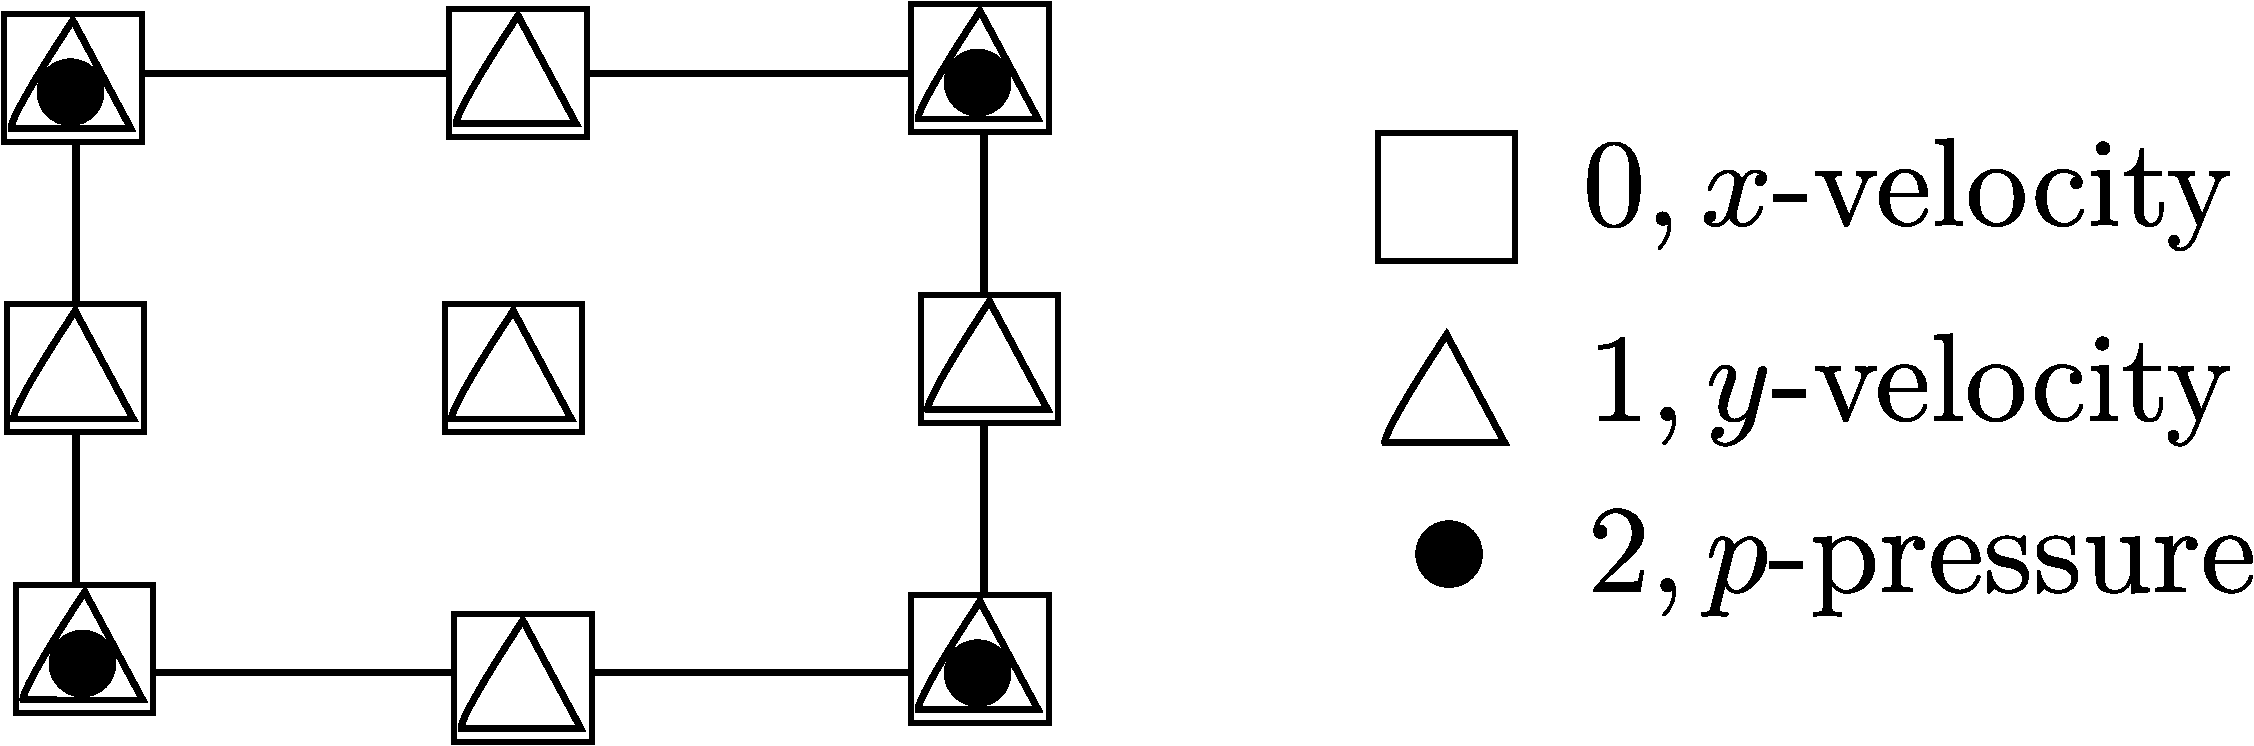
\includegraphics[width=0.9\textwidth]{./pic/taylorhood_dof_classification.pdf}
\caption{Elemental DOF type classification for \texttt{oomph-\allowbreak lib}'s 
\texttt{Q\allowbreak TaylorHood\allowbreak Element<2>} elements.}
\label{fig:2DTH_DOF_classification}
\end{figure}

\subsubsection{The role of meshes}

Within the block preconditioning framework, each mesh acts as a container for 
a set of DOF type classifications. All elements in the same mesh \emph{must} 
return the same \texttt{ndof\_\allowbreak types()} value. If two different 
element types are in the same mesh, and their \texttt{ndof\_\allowbreak types()}
does indeed return the same number, then their elemental DOF type 
classifications will be treated as the same type. For example, recall in 
Figure \ref{fig:2DTH_DOF_classification} that the elemental DOF types 
classification for \texttt{Q\allowbreak TaylorHood\allowbreak Element<2>} 
elements are as follows:
\begin{itemize}
  \item \texttt{0} $x$-velocity
  \item \texttt{1} $y$-velocity
  \item \texttt{2} $p$-pressure
\end{itemize}
If we wish to constrain the flow along a boundary, we can attach the 
\texttt{Face\allowbreak Element}s 
\texttt{Impose\allowbreak Parallel\allowbreak Outflow\allowbreak Element<ELEMENT>} 
along the appropriate boundary as shown in the demo problem: Steady 
finite-Reynolds-number flow through an iliac bifurcation, these 
\texttt{Face\allowbreak Element}s classifies the `bulk' velocity DOF types 
as well as it's own DOF type as shown in Figure 
\ref{fig:2DFACE_DOF_classification}.
\begin{figure}[H]
\centering
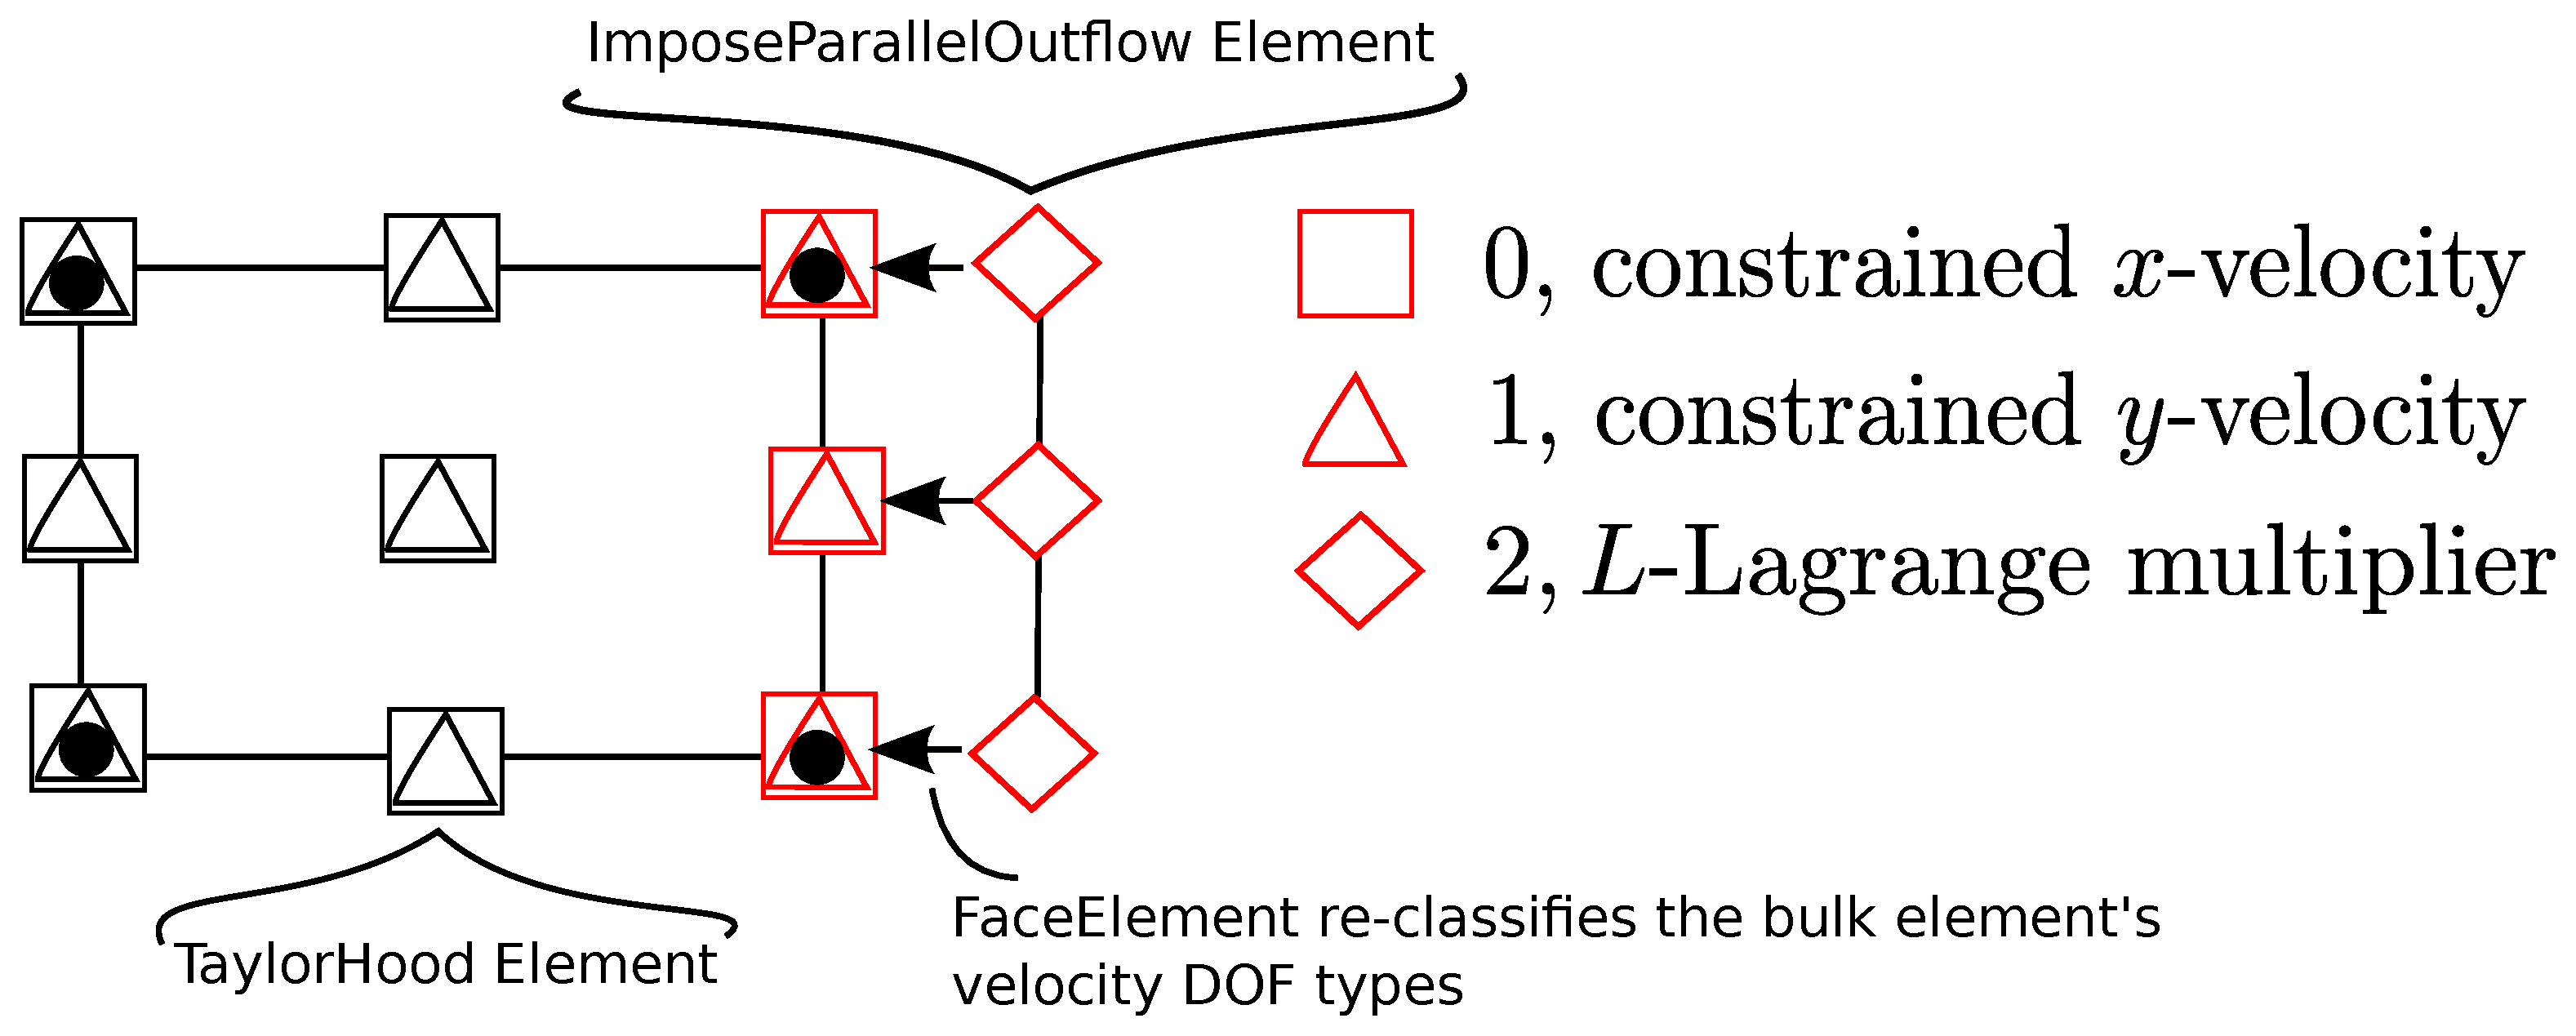
\includegraphics[width=0.9\textwidth]{./pic/faceelemenet_dof_classification.pdf}
\caption{Elemental DOF type classification for \texttt{oomph-\allowbreak lib}'s 
 \texttt{Impose\allowbreak Parallel\allowbreak Outflow\allowbreak Element<ELEMENT>} elements.}
\label{fig:2DFACE_DOF_classification}
\end{figure}

Although the \texttt{ndof\_\allowbreak types()} for these two different elements are the same,
there are clearly six distinct DOF types. To ensure that the block 
preconditioning framework treats these as different DOF types, we must have two
meshes for the two different type of elements. If we put the two elements types
in the same mesh, then the block preconditioning framework will not distinguish
between the two \texttt{0} elemental DOF types, i.e. $x$-velocity is the same as 
constrained $x$-velocity. The same applies to the remaining two elemental 
DOF types \texttt{1} and \texttt{2}. Within the block preconditioning framework, 
there is a built-in check to throw an error if a mesh passed to the framework 
contains multiple types of elements. This check can be avoided by setting the 
optional argument 
\texttt{allow\_\allowbreak multiple\_\allowbreak element\_\allowbreak type\_\allowbreak in\_\allowbreak mesh} 
when calling the function \texttt{set\_\allowbreak mesh(...)} to \texttt{true}. 
In this case, the framework will check if the \texttt{ndof\_\allowbreak types()} 
of all the elements of the same mesh are the same.

\subsubsection{Block preconditioner DOF types}
The information contained in different meshes allow the BPF to order the elemental
DOF types (note that the function \texttt{ndof\_\allowbreak types()} provides 
the block offset). For example, consider the above \texttt{vmtk} RAYFIX problem, 
the first mesh (the bulk mesh) contain elements with elemental DOF types 
\texttt{0}, \texttt{1} and \texttt{2} for the $x$, $y$-velocities and pressure
respectively. The second mesh (the surface mesh) contain elements with elemental
DOF types \texttt{0}, \texttt{1} and \texttt{2} for the $x$, $y$-constrained 
velocities and Lagrange multiplier respectively. Let $N$ be the 
number of meshes, $N_i$ be the number of elemental DOF types in mesh $i$,
$E_i = 0, \ldots N_i - 1$ be the elemental DOF types in mesh $i$, $B_{i,E_i}$ 
be the corresponding block preconditioner DOF types. Then the relationship 
between the block preconditioner DOF type $B_{i,E_i}$ and elemental DOF type
$E_i$ is given by
\begin{equation*}
  B_{i,E_i} = E_i + \sum_{i=0}^{N - 1} N_i, \quad \mbox{for } E_i = 0,\ldots N_i.
\end{equation*}
Figure \ref{fig:elemental_to_block_dof_classification} shows the mapping between
elemental DOF types and block preconditioner DOF types for the example above.
\begin{figure}[H]
\centering
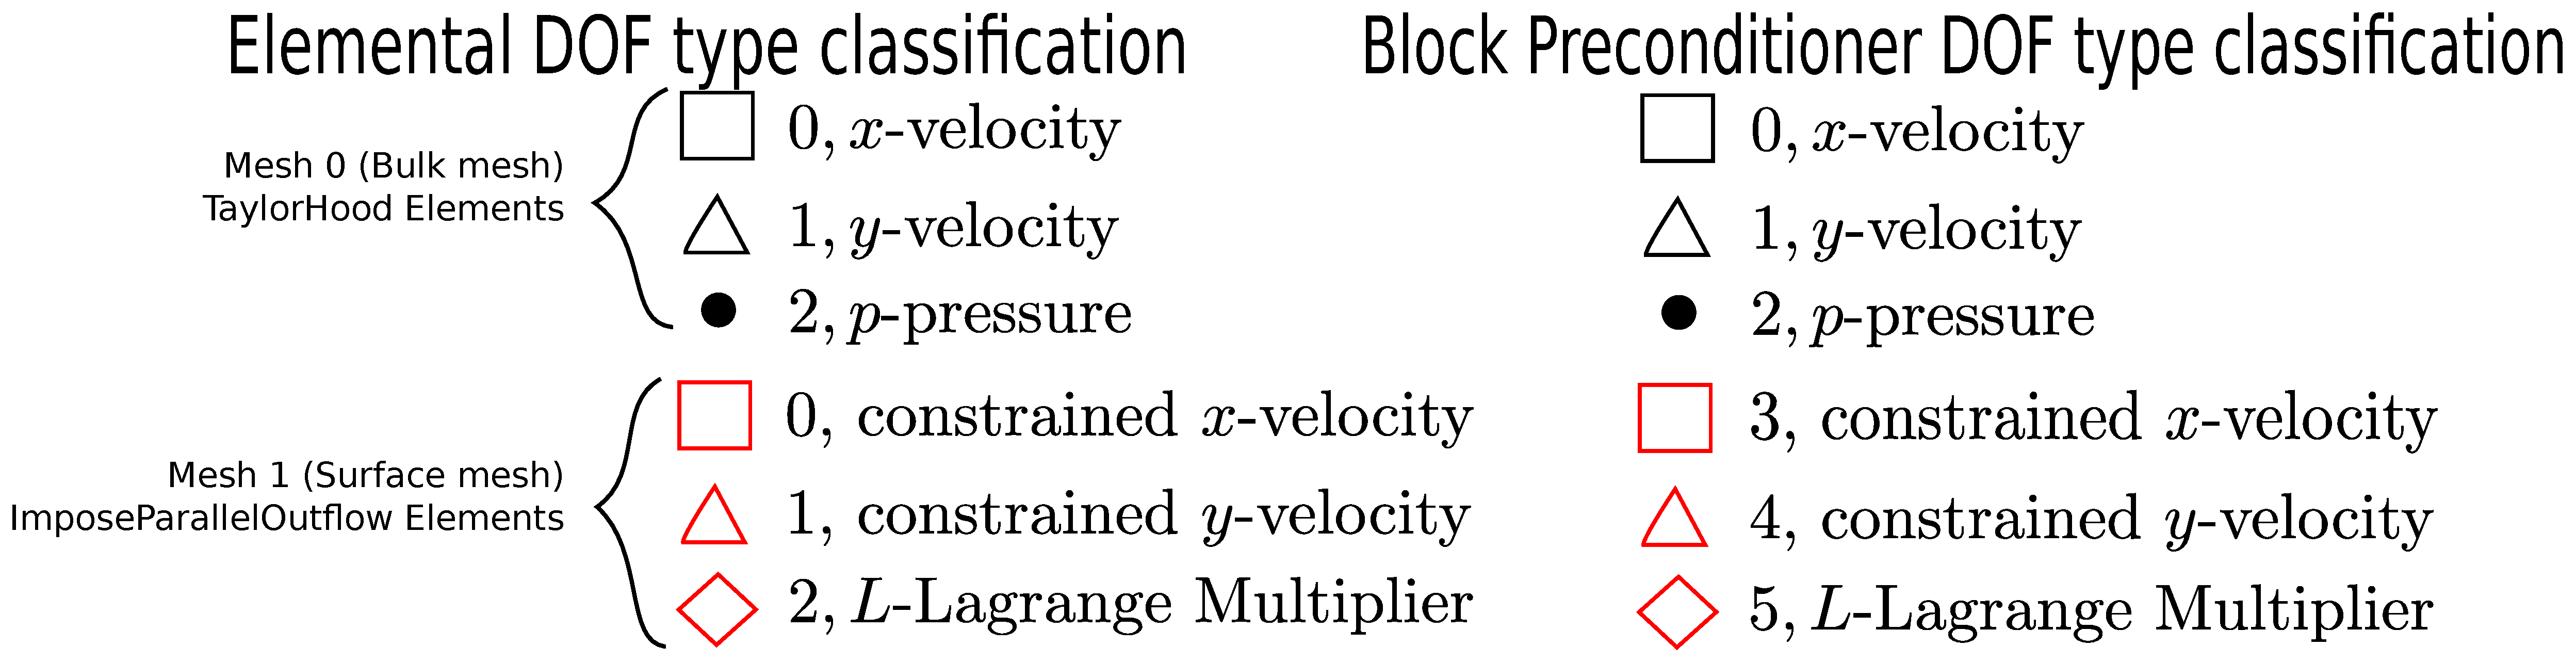
\includegraphics[width=1\textwidth]{./pic/elemental_to_block_dof_classification.pdf}
\caption{Relationship between the classification of elemental DOF types and block
         preconditioner DOF types.}
\label{fig:elemental_to_block_dof_classification}
\end{figure}

It is important to note that within the BPF, when multiple meshes are used, the
block preconditioner DOF types admit to a two-level ordering: first by the mesh 
they belong to, and then by the elemental DOF type within the mesh. To this end, 
where the ordering of the block preconditioner DOF types matters (such as the 
LSC preconditioner), the block preconditioner should handle the ordering of the 
meshes, the user should use functions such as 
\texttt{set\_\allowbreak navier\_\allowbreak stokes\_\allowbreak mesh(...)}
in the case of the 
\texttt{Navier\allowbreak Stokes\allowbreak Schur\allowbreak Complement\allowbreak Preconditioner} 
since the LSC preconditioner know where the Navier-Stokes mesh need to be in 
the order of the meshes. We refer the ordering of the preconditioner DOF types, 
determined by the elemental DOF type and the ordering of the meshes, the 
\emph{natural ordering} of the preconditioner DOF types. For the above example, the natural ordering of the preconditioner DOF
types would be:
\begin{itemize}
 \item \verb+0+ $x$-velocity
 \item \verb+1+ $y$-velocity
 \item \verb+2+ $p$-pressure
 \item \verb+3+ constrained $x$-velocity
 \item \verb+4+ constrained $y$-velocity
 \item \verb+5+ $L$-Lagrange multiplier
\end{itemize}

Note: Each DOF can be classified more than once. If this is the case, then the classification will be the last mesh visited by the block preconditioning framework. This should not be an issue if you do not have discontinuous boundary conditions.

\subsubsection{Block types}
The block types are the blocks of sub-matrices the block preconditioner works with. Block types may contain more than one preconditioner DOF types or be as fine grain as the number of preconditioner DOF types. Note: There can not be more block types than there are preconditioner DOF types. For example, in case of the the LSC preconditioner (in 2D) we have three DOF types ($x$ , $y$-velocities, and pressure), but the preconditioner only distinguishes between velocity and pressure DOF types, thus we have two block types (velocity block and pressure block). The setup of the block types are handled by the function... \verb+block_setup(...)+. The setup of the blocks and DOF types will be discussed in more detail later on.


%%%% MASTER AND SUBSIDIARY PRECONDITIONER
\subsection{Master and Subsidiary Preconditioners\label{sec:master_and_subsidiary_preconditioners}}
Consider the again the LSC Navier-Stokes preconditioner.
If we decide to approximate the $\mathbf{F}$ block (the momentum block) by it's diagonal blocks, we can pass the block diagonal preconditioner (discussed in (Distributed) General-Purpose Block Preconditioners) to the LSC preconditioner to use as a subsidiary preconditioner via the function \verb+set_f_preconditioner(...)+. We can do the same with the pressure system with the function \verb+set_p_preconditioner(...)+. We refer to these preconditioners as subsidiary preconditioners. \verb+Oomph-lib+'s block preconditioning framework facilitates the the reuse of existing preconditioners as subsidiary preconditioners.

It is important to note that we do not need to consider the \verb+block structure+ of subsidiary block preconditioners when developing master preconditioners. However, the master preconditioner must be aware of the preconditioner DOF type ordering of the subsidiary preconditioner. For example, if the LSC preconditioner is a subsidiary preconditioner (as is the case of the FSI preconditioner), the FSI preconditioner must ensure that the last DOF type given to the LSC preconditioner is the pressure DOF type, and the ones before that are the velocity DOF types.

There is only one `true' master preconditioner, the rest are all subsidiary preconditioners, each subsidiary preconditioner holds a pointer to the preconditioner one level up in the hierarchy. Say, there are three preconditioners, $P1$, $P2$ and $P3$. If we use $P2$ to solve a subsidiary system in $P1$, and $P3$ to solve a subsidiary system in $P2$, then it could be said that $P1$ is the master preconditioner for $P2$, and $P2$ is a master preconditioner for $P3$. However, because $P2$'s \verb+Master_block_preconditioner_pointer_pt+ is not null, it is automatically classed as a subsidiary preconditioner. Only the true master preconditioner (so that the \verb+Master_block_preconditioner_pt+ is null) holds all the information about the DOF types and look-up schemes. If a subsidiary preconditioner requires information held only by the master preconditioner, it will go to it's `master' preconditioner. If this `master' preconditioner is a subsidiary preconditioner, it will again go up the hierarchy to it's master preconditioner.

%%%%%%%%%%%%%%%%%%%%%%%%%%%%%%%%%%%%%%%%%%%%%%%%%%%%%
%%% USING THE SIMPLE DIAGONAL BLOCK PRECONDITIONER
%%%%%%%%%%%%%%%%%%%%%%%%%%%%%%%%%%%%%%%%%%%%%%%%%%%%%
\section{Using the Simple Block Preconditioner\label{sec:using_the_simple_block_preconditioner}}

We begin our discussion of the implementation details by demonstrating how to use the preconditioner (implemented in the class \verb+SimpleBlockDiagonalPreconditioner+) in an actual driver code 

(\verb+two_d_linear_elasticity_with_simple_block_diagonal_preconditioner.cc+).

In the problem constructor, we construct the solver and preconditioner combination. We specify the GMRES iterative solver, and, if available, use the distributed version implemented in \verb+TrilinosAztecOOSolver+.
\lstset{numberstyle=\scriptsize,breaklines=true, numbers=left, stepnumber=2, frame=single,basicstyle=\ttfamily\scriptsize, showstringspaces=false, language=C++}
\lstinputlisting[firstnumber=348, firstline=348, lastline=361]{./code/two_d_linear_elasticity_with_simple_block_diagonal_preconditioner.cc}
Then we construct an instance of the preconditioner. This linear elasticity problem contains one types of element used for preconditioning (see section \ref{sec:block_preconditionable_elements}). There also exists \verb+LinearElasticityTractionElement+, but in this case the block preconditioner does not require the surface mesh since the bulk mesh contains all the DOFs that needs to be classified and \verb+MyLinearElasticityElement+ does classify all the DOF in the bulk mesh. We store
the different element types in seperate meshes. Only the bulk mesh is passed to the preconditioner. Finally, the preconditioner is passed to the 
solver.
\lstset{numberstyle=\scriptsize,breaklines=true, numbers=left, stepnumber=2, frame=single,basicstyle=\ttfamily\scriptsize, showstringspaces=false, language=C++}
\lstinputlisting[firstnumber=363,firstline=363, lastline=373]{./code/two_d_linear_elasticity_with_simple_block_diagonal_preconditioner.cc}
In the main function,
\lstset{numberstyle=\scriptsize,breaklines=true, numbers=left, stepnumber=2, frame=single,basicstyle=\ttfamily\scriptsize, showstringspaces=false, language=C++}
\lstinputlisting[firstnumber=450,firstline=450, lastline=454]{./code/two_d_linear_elasticity_with_simple_block_diagonal_preconditioner.cc}
we create an instance of the  problem which problem can now be solved in the normal \verb+oomph-lib+ fashion:
\lstset{numberstyle=\scriptsize,breaklines=true, numbers=left, stepnumber=2, frame=single,basicstyle=\ttfamily\scriptsize, showstringspaces=false, language=C++}
\lstinputlisting[firstnumber=466,firstline=466, lastline=480]{./code/two_d_linear_elasticity_with_simple_block_diagonal_preconditioner.cc}


%%%%%%%%%%%%%%%%%%%%%%%%%%%%%%%%%%%%%%%%%%%%%%%%%%%%%
%%% IMPLEMENTING A BLOCK DIAGONAL PRECONDITIONER
%%%%%%%%%%%%%%%%%%%%%%%%%%%%%%%%%%%%%%%%%%%%%%%%%%%%%
\section{The implementation of a block diagonal preconditioner\label{sec:the_implementation_of_a_block_diagonal_preconditioner}}

We discuss the implementation of a block preconditioner within
\verb+oomph-lib+'s block preconditioning framework. In particular, we will address three fundamental tasks:
\begin{itemize}
\item How to identify and classify the DOFs in the underlying \verb+Problem+.
\item How to extract subsidiary matrix blocks from the full Jacobian.
\item How to recycle existing preconditioning operators within new preconditioners.
\end{itemize}

We implement the block diagonal preconditioner in the
class \verb+SimpleBlockDiagonalPreconditioner+. This class inherits
from the base class \verb+BlockPreconditioner+ which provides the generic 
functionality required for common block preconditioning operations.
\lstset{numberstyle=\scriptsize,breaklines=true, numbers=left, stepnumber=2, frame=single,basicstyle=\ttfamily\scriptsize, showstringspaces=false, language=C++}
\lstinputlisting[firstnumber=53,firstline=53, lastline=55]{./code/simple_block_preconditioners.h}
This preconditioner requires a \verb+Vector+ of pointers to \verb+Preconditioner+s for each diagonal block matrix.
\lstinputlisting[firstnumber=97,firstline=97, lastline=99]{./code/simple_block_preconditioners.h}

%%%% CONSTRUCTOR FOR BLOCK DIAGONAL PRECONDITIONER
\subsection{Constructor for block diagonal preconditioner\label{sec:constructor_for_block_diagonal_preconditioner}}
The constructor is usually used to initialised variables. In this case, there is nothing to initialise.
\lstinputlisting[firstnumber=59,firstline=59, lastline=62]{./code/simple_block_preconditioners.h}

%%%% CONSTRUCTOR FOR BLOCK DIAGONAL PRECONDITIONER
\subsection{setup(...) for block diagonal preconditioner\label{sec:block_diagonal_preconditioner_setup}}

Like all preconditioners, \verb+BlockPreconditioners+ have two key
functions, \verb+setup(...)+ and \verb+preconditioner_solve(...)+ both of which are discussed in more detail in the \verb+oomph-lib+ Linear Solvers Tutorial [CITE]. We begin by considering the function \verb+setup(...)+.
\lstinputlisting[firstnumber=107,firstline=107, lastline=109]{./code/simple_block_preconditioners.h}
At the simplest level, \verb+Meshes+ are just containers for elements. To reiterate section \ref{sec:dof_types_and_block_types}, storing different element type in separate meshes enables the \verb+BlockPreconditioner+ to differentiate between the elemental DOF types of different element types. The order of the meshes determine the order of the preconditioner DOF types.
Therefore, in more sophisticated preconditioners, the preconditioner usually handle the calls to \verb+set_nmesh(...)+ and \verb+set_mesh(...)+ functions. For this simplistic case, the functions \verb+set_nmesh(...)+ and \verb+set_mesh(...)+ were called in the driver code (see section \ref{sec:using_the_simple_block_preconditioner}).

Passing the meshes to \verb+BlockPreconditioner+ gives the framework access to the
meshes and allows the preconditioner write access to the number of DOF types associated with the elements in each mesh.

\subsubsection{block\_setup(...)\label{sec:block_setup}}
The next step is to define a mapping from DOF number to block
number. This preconditioner's block type is as fine grain as the preconditioner DOF types. To see this, recall, if the Jacobian (partitioned into DOF types) takes the form 
\begin{equation*}
J =
\begin{bmatrix}
S_{xx}&S_{xy} \\
S_{yx}&S_{yy}
\end{bmatrix},
\end{equation*}
then the preconditioner is
\begin{equation*}
P_{diag} =
\begin{bmatrix}
S_{xx}& \\
      &S_{yy}
\end{bmatrix}.
\end{equation*}
It is clear that the blocks the preconditioner works with has to be as fine grain as the DOF types. This is achieved by calling the function \verb+block_setup(...)+ with no arguments. By default, this has the same effect as calling \verb+block_setup(...)+ with the identity \verb+dof_to_block_map+ Vector \verb+=+ \verb+[0 1]+.
\lstinputlisting[firstnumber=111,firstline=111, lastline=112]{./code/simple_block_preconditioners.h}

For this simple block diagonal preconditioner, there is method of changing the \verb+dof_to_block_map+ Vector. There exists a more sophisticated version of the block diaginal preconditioner in the class \verb+GeneralPurposeBlockPreconditioner+, where there exists a function

\noindent\verb+set_dof_to_block_map(Vector<unsigned>& dof_to_block_map)+
to change the \verb+dof_to_block_map+ from the default. Subtilties of the \verb+dof_to_block_map+ Vector is discussed below.

\subsubsection{block\_setup(...): Combining DOF types\label{sec:block_setup_combining_dof_types}}
If we want a block type to consist of more than one preconditioner DOF type, then we can provide a \verb+dof_to_block_map+ to the function \verb+block_setup(...)+ describing the mapping we want. For example, if we extend the example above so there are three DOF types,
\begin{equation*}
J =
\begin{bmatrix}
S_{xx}&S_{xy}&S_{xz} \\
S_{yx}&S_{yy}&S_{yz} \\
S_{zx}&S_{zy}&S_{zz}
\end{bmatrix},
\end{equation*}
and instead of simply using the diagonal blocks, we want to use a block preconditioner of the following form
\begin{equation*}
\tilde{P}_{diag} =
\begin{bmatrix}
S_{xx}&S_{xy}&       \\
S_{yx}&S_{yy}&       \\
      &      &S_{zz}
\end{bmatrix}.
\end{equation*}
That is, we want to group the first two preconditioner DOF types as one block type and the last preconditioner DOF type as a separate block type. This is achieved by passing the \verb+dof_to_block_map+ \verb+=+ \verb+[0 0 1]+ to the function \verb+block_setup(...)+, we see a similar \verb+dof_to_block_map+ in the implementation of the LSC preconditioner. It is important to note that although the (in C++ index notation) block (0,0) consists of preconditioner DOF types 
$\displaystyle
\begin{bmatrix}
S_{xx}&S_{xy} \\
S_{yx}&S_{yy} 
\end{bmatrix}
$, it is not gauranteed that the DOF types are grouped in such a manner in the (0,0) block.

\subsubsection{block\_setup(...): Re-ordering DOF types\label{sec:block_setup_reordering_dof_types}}
Continuing from the example above, the natural ordering of the preconditioner DOF types (determined by the ordering of the elemental DOF types and the order of the meshes added to the block preconditioner as decribed in section \ref{sec:dof_types_and_block_types}) is:
\begin{center}
    \begin{tabular}{ | r | c c c |}
    \hline
    DOF type name: & $S_{x}$ & $S_{y}$ & $S_{z}$ \\ 
    Natural ordering: & 0 & 1 & 2 \\ 
    \hline
    \end{tabular}
\end{center}
We have named the DOF types so facilitate the discussion. Suppose we want to re-order the DOF types such that we have the following block order:
\begin{center}
    \begin{tabular}{ | r | c c c |}
    \hline
    New block order: & $S_{z}$ & $S_{x}$ & $S_{y}$ \\ 
    \hline
    \end{tabular}
\end{center}
Then the \verb+dof_to_block_map+ \verb+Vector+ will be
\begin{center}
    \begin{tabular}{ | r | c c c |}
    \hline
    \verb+dof_to_block_map+: & 1 & 2 & 0 \\ 
    \hline
    \end{tabular}
\end{center}
The index of the \verb+dof_to_block_map+ Vector is the DOF type you want to move, then ask yourself `where do I want to move this DOF type to?', put this value into the current position in the \verb+dof_to_block_map+ Vector.

Combining this with the previous concept, it is possible to create a preconditioner of the form
\begin{equation*}
\tilde{P}_{diag} =
\begin{bmatrix}
S_{zz}&S_{zx}&       \\
S_{xz}&S_{xx}&       \\
      &      &S_{yy}
\end{bmatrix}
\end{equation*}
with the \verb+dof_to_block_map+ Vector \verb+[0 1 0]+.

%%%% Set up the subsidiary preconditioners
\subsubsection{Set up subsidiary preconditioners\label{sec:set_up_subsidiary_preconditioners}}
The next step is to set up the subsidiary preconditioners. We use the \verb+SuperLU+ preconditioner for all the subsidiary systems, we require as many subsidiary preconditioners as there are the number of blocks that the block preconditioner is working with. First we create a new instances of the of \verb+SuperLUPreconditioner+ for every block.
\lstinputlisting[firstnumber=114,firstline=114, lastline=124]{./code/simple_block_preconditioners.h}
Now we extract the diagonal blocks and call the \verb+setup(...)+ function of the subsidiary preconditioners.
\lstinputlisting[firstnumber=126,firstline=126, lastline=138]{./code/simple_block_preconditioners.h}

%%%% PRECONDITIONER SOLVE FOR BLOCK DIAGONAL PRECONDITIONER
\subsection{Preconditioner solve for block diagonal preconditioner\label{sec:preconditioner_solve_for_block_diagonal_preconditioner}}
Next we consider the \verb+preconditioner_solve(...)+ function which applies the action of the preconditioner to the input vector $\mathbf{y}$ and returns the result in $\mathbf{z}$.
\lstinputlisting[firstnumber=142,firstline=142, lastline=147]{./code/simple_block_preconditioners.h}
In this section, we implement the application of the preconditioner as described in the section \ref{sec:theoretical_background}. First we split the rhs vector into sub-vectors, re-arranged to match the block order of the preconditioner blocks.
\lstinputlisting[firstnumber=149,firstline=149, lastline=152]{./code/simple_block_preconditioners.h}
Next we loop through the LU decompositions stored in the \verb+Diagonal_block_preconditioner_pt+, and apply the subsidiary preconditioners.
\lstinputlisting[firstnumber=157,firstline=157, lastline=163]{./code/simple_block_preconditioners.h}
Finally we return the solution back into $\mathbf{z}$ in the correct DOF order.
\lstinputlisting[firstnumber=165,firstline=165, lastline=166]{./code/simple_block_preconditioners.h}


%%%%%%%%%%%%%%%%%%%%%%%%%%%%%%%%%%%%%%%%%%%%%%%%%%%%%
%%% LSC BLOCK PRECONDITIONER
%%%%%%%%%%%%%%%%%%%%%%%%%%%%%%%%%%%%%%%%%%%%%%%%%%%%%
\section{LSC block preconditioner\label{sec:lsc_block_preconditioner}}
Theoretical dicussion of the LSC preconditioner can be found in "Finite Elements and Fast Iterative Solvers with Applications in Incompressible Fluid 
Dynamics" by Howard C. Elman, David J. Silvester, and Andrew J. Wathen,
published by Oxford University Press, 2006.

In this section, we partially follow the \verb+oomph-lib+ LSC tutorial [CITE oomph-lib lsc tutorial], where we take a closer look at the implementation details to address the following concepts:
\begin{itemize}
\item Non trivial grouping of preconditioner DOF types into block types.
\item Setting up \verb+MatrixVectorProduct+s within the block preconditioning framework.
\item Subsidiary block preconditioners:
 \begin{itemize}
 \item The \verb+dof_map+ for the \verb+turn_into_subsidiary_block_preconditioner(...)+ function.
 \item Modification to the \verb+preconditioner_solve(...)+ function.
 \end{itemize}
\end{itemize}

%%%% LSC theory
\subsection{Theory\label{sec:lsc_theory}}
\verb+oomph-lib+ currently provides two types of (LBB-stable)
Navier-Stokes elements: Taylor-Hood (Q2Q1) and Crouzeix-Raviart
(Q2Q-1) elements. These contain two distinct types of degrees of freedom,
namely the velocities and pressures.

The least-squares commutator (LSC; formerly BFBT) Navier-Stokes 
preconditioner employs \verb+oomph-lib+'s block-preconditioning framework
to (formally) re-order the linear system to be solved during the
Newton iteration into 2x2 blocks, corresponding to the velocity 
and pressure unknowns. We note that all velocity components are 
treated as a single block of unknowns. The linear system
therefore has the following block structure
\begin{equation*}
\begin{bmatrix}
{\bf F} & {\bf G} \\ {\bf D} & {\bf 0} 
\end{bmatrix}
\begin{bmatrix}
{\bf z}_u \\ {\bf z}_p
\end{bmatrix} 
 =
\begin{bmatrix}
{\bf r}_u \\ {\bf r}_p
\end{bmatrix} 
.
\end{equation*}
Here $\mathbf{F}$ is the momentum block, $\mathbf{G}$ the
discrete gradient operator, and $\mathbf{D}$ the discrete
divergence operator. (For unstabilised elements, we have 
$\mathbf{D} = \mathbf{G}^T$ and in much of the literature
the divergence matrix is denoted by $\mathbf{B}$.)

An "exact" preconditioner would solve this system exactly and thus
ensure the convergence of any iterative linear solver in a single 
iteration. However, the application of such a preconditioner
would, of course, be exactly as expensive as a direct solve.
The LSC/BFBT preconditioner replaces the exact Jacobian by 
a block-triangular approximation
\begin{equation*}
\begin{bmatrix}
{\bf F} & {\bf G} \\ {\bf 0} & -{\bf M}_s 
\end{bmatrix} 
\begin{bmatrix}
{\bf z}_u \\ {\bf z}_p
\end{bmatrix} 
=
\begin{bmatrix}
{\bf r}_u \\ {\bf r}_p
\end{bmatrix}
,
\end{equation*}
where $\mathbf{M}_s$ is an approximation to the pressure 
Schur-complement $\mathbf{S}=\mathbf{D} \mathbf{F}^{-1}\mathbf{G}$.
This system can be solved in two steps:
\begin{enumerate}
\item Solve the second row for $\mathbf{z}_p$ via
   \begin{equation*}
   \mathbf{z}_p = - \mathbf{M}_s^{-1} \mathbf{r}_p
   \end{equation*}
\item Given $\mathbf{ z}_p$, solve the first row for $\mathbf{z}_u$ via
   \begin{equation*}
   \mathbf{z}_u = \mathbf{F}^{-1} \left( \mathbf{r}_u - \mathbf{G} \mathbf{z}_p \right)
   \end{equation*}
\end{enumerate}
In the LSC/BFBT preconditioner, the action of the inverse pressure
Schur complement 
\begin{equation*}
\mathbf{z}_p = - \mathbf{M}_s^{-1} \mathbf{r}_p
\end{equation*}
is approximated by
\begin{equation*}
\mathbf{z}_p = - 
\big(\mathbf{D} \widehat{\mathbf Q}^{-1}{\mathbf G} \big)^{-1}
\big({\mathbf D} \widehat{\mathbf Q}^{-1}{\mathbf F} \widehat{\mathbf Q}^{-1}{\mathbf G}\big) 
\big({\mathbf D} \widehat{\mathbf Q}^{-1}{\mathbf G} \big)^{-1}
{\mathbf r}_p,
\end{equation*}
where  $ \widehat{\mathbf Q}$ is the diagonal of the velocity
mass matrix. The evaluation of this expression involves
two linear solves involving the matrix
\begin{equation*}
{\mathbf P} = \big({\mathbf D} \widehat{\mathbf Q}^{-1}{\mathbf G} \big)
\end{equation*}
which has the character of a matrix arising from the discretisation 
of a Poisson problem on the pressure space. We also have
to evaluate matrix-vector products with the matrix 
\begin{equation*}
{\mathbf E}={\mathbf D}\widehat{\mathbf Q}^{-1}{\mathbf F}\widehat{\mathbf Q}^{-1}{\mathbf G}
\end{equation*}
In our implementation of the preconditioner, the linear systems
can either be solved "exactly", using \verb+SuperLU+ (in its incarnation
as an exact preconditioner; this is the default) or by any 
other \verb+Preconditioner+ (interpreted as an "inexact solver")
specified via the access functions
\begin{verbatim}
NavierStokesSchurComplementPreconditioner::set_f_preconditioner(...)
\end{verbatim}
or 
\begin{verbatim}
NavierStokesSchurComplementPreconditioner::set_p_preconditioner(...)
\end{verbatim}

%%%% Implementation details
\subsection{Implementation\label{sec:lsc_implementation}}
In this section we focus on aspect of the implementation relevant to the 
discussion of the block preconditioning framework.
Let \verb+dim+ be the spatial dimension of the problem, then \verb+NavierStokesSchurComplementPreconditioner+ expects 
\verb+dim+ + 1 preconditioner DOF types, \verb+dim+ number of DOF types corresponds to the velocity DOF types and 1 DOF type for the pressure. 

\subsubsection{setup(...) for the LSC preconditioner\label{sec:lsc_implementation_setup}}
We need to group the velocity DOF types as one block type and the pressure DOF type as one DOF type. This is achieved by setting the first \verb+dim+ entries of the \verb+dof_to_block_map+ Vector to 0 and the last entry to 1.
\lstinputlisting[firstnumber=235,firstline=235, lastline=238]{./code/navier_stokes_preconditioners.cc}
For example, in two dimensions, the natural ordering of the DOF types and the \verb+dof_to_block_map+ Vector is given below.
\begin{center}
    \begin{tabular}{ | r | c c c |}
    \hline
    DOF type name: & $u$ & $v$ & $p$ \\ 
    Natural ordering: & 0 & 1 & 2 \\ 
    \verb+dof_to_block_map+: & 0 & 0 & 1 \\ 
    \hline
    \end{tabular}
\end{center}


The implementation follows the theory in section \ref{sec:lsc_theory}. We highlight important points to note when implementing a new preconditioner. 


When setting up a \verb+MatrixVectorProduct+, it is important to use the setup function \verb+setup_matrix_vector_product(...)+. The first argument is a pointer to the \verb+MatrixVectorProduct+, the second is a pointer to the matrix we wish to set up with, the third is an unsinged value indicating the block vector which the matrix needs to be multiplied by. This ensures that the column distribution of the \verb+MatrixVectorProduct+ is set up properly.
\lstinputlisting[firstnumber=493,firstline=493, lastline=494]{./code/navier_stokes_preconditioners.cc}

If the $\mathbf{F}$ preconditioner is a block preconditioner (used to solve the system $\mathbf{z}_u = \mathbf{F}^{-1} \left( \mathbf{r}_u - \mathbf{G} \mathbf{z}_p \right)$), then we must call the function 

\noindent\verb+turn_into_subsidiary_block_preconditioner(...)+ of the $\mathbf{F}$ preconditioner. This function takes the pointer of the `master' preconditioner (in this sense, master is just one level higher in the block preconditioning framework hierarchy), and a Vector describing a mapping of preconditioner DOF types of the master preconditioner and the subsidiary preconditioner. Then the \verb+setup(...)+ function of the subsidiary preconditioner is called with a pointer to the whole jacobian (via the access function \verb+matrix_pt()+). If the $\mathbf{F}$ preconditioner is not a block preconditioner, then we do the same as we did in the simple block diagonal preconditioner case.
\lstinputlisting[firstnumber=577,firstline=577, lastline=596]{./code/navier_stokes_preconditioners.cc}
The \verb+dof_map+ Vector is different from the \verb+dof_to_block_map+ Vector. The \verb+dof_to_block_map+ Vector describes the mapping of the preconditioner DOF types to block types within the same block preconditioner, as such, this Vector must have the same size as the number of DOF types the preconditioner expects to be working with. The \verb+dof_map+ Vector describes the mapping between the DOF types of a master preconditioner with it's subsidiary preconditioner. Re-ordering DOF types of the subsidiary preconditioner using the \verb+dof_map+ Vector is possible and will be demonstrated in the implementation of the Lagrangian preconditioner discussed later in this document.


\subsubsection{preconditioner\_solve(...) for the LSC preconditioner\label{sec:lsc_implementation_precsolve}}
The \verb+preconditioner_solve(...)+ function for the LSC preconditioner follows the theory discussed in section \ref{sec:lsc_theory}. When block preconditioner are used as subsidiary preconditioners, we DO NOT return the block vector, as this is handled by the subsidiary block preconditioner.
\lstinputlisting[firstnumber=785,firstline=785, lastline=796]{./code/navier_stokes_preconditioners.cc}


%%%%%%%%%%%%%%%%%%%%%%%%%%%%%%%%%%%%%%%%%%%%%%%%%%%%%
%%% LAGRANGIAN BLOCK PRECONDITIONER
%%%%%%%%%%%%%%%%%%%%%%%%%%%%%%%%%%%%%%%%%%%%%%%%%%%%%
\section{Lagrangian block preconditioner\label{sec:lagrangian_block_preconditioner}}
In this section, we use the implementation of the Lagrangian preconditioner to address the following concepts:
\begin{itemize}
\item Non-trivial re-ordering of block types.
\item Non-trivial re-ordering of subsidiary DOF types.
\item Set precomputed preconditioner blocks for subsidiary block preconditioners.
\end{itemize}
As with previous examples, we highlight the key concepts and neglect the finer implementation details of the preconditioner for the specific problem. The code is (as always) well documented and can be worked through with the theory at hand.
%%%% LSC theory
\subsection{Theory\label{sec:lgr_theory}}
Suppose we want to impose parallel outflow along a boundary, we attach the block preconditionable elements \verb+ImposeParallelOutflowElement+ along the said boundary as discussed in section \ref{sec:dof_types_and_block_types}. This will result in a jacobian of the following block form (partitioned by DOF types):
\renewcommand{\arraystretch}{1.2}
\begin{equation}
\newcommand*{\temp}{\multicolumn{1}{r|}{}}
\left[
\begin{array}{cccccccc}
F_{xx}&F_{xy}&F_{x\hat{x}}&F_{x\hat{y}}& \temp &(B_x)^T&\temp & \\ 
F_{yx}&F_{yy}&F_{y\hat{x}}&F_{y\hat{y}}& \temp &(B_{y})^T&\temp & \\
F_{\hat{x}x}&F_{\hat{x}y}&F_{\hat{x}\hat{x}}&F_{\hat{x}\hat{y}}& \temp &(B_{\hat{x}})^T&\temp & M_x\\
F_{\hat{y}x}&F_{\hat{y}y}&F_{\hat{y}\hat{x}}&F_{\hat{y}\hat{y}}& \temp &(B_{\hat{y}})^T&\temp &M_y \\ 
  \cline{1-7}
B_x&B_{y} &B_{\hat{x}} &B_{\hat{y}} & \temp &  &\temp & \\ 
  \cline{1-8}
  & & M_x & M_y&       &  &\temp & \\
\end{array}
\right]
\left[
\begin{array}{c}
\delta \bar{u}_x \\
\delta \bar{u}_y \\
\delta \bar{u}_{\hat{x}} \\
\delta \bar{u}_{\hat{y}} \\
\delta \bar{p} \\
\delta \bar{l} \\
\end{array}
\right]
=
\left[
\begin{array}{c}
\delta \bar{r}_x \\
\delta \bar{r}_y \\
\delta \bar{r}_{\hat{x}} \\
\delta \bar{r}_{\hat{y}} \\
\delta \bar{r}_p \\
\delta \bar{r}_l \\
\end{array}
\right],
\end{equation}
\renewcommand{\arraystretch}{1}
where the block vector $[\bar{u}_x \, \bar{u}_{\hat{x}}]^T$ contains the $x$ coordinates of the unknown nodal positions. Similarly, the block vector $[\bar{u}_y \, \bar{u}_{\hat{y}}]^T$ contains the $x$ coordinates of the unknown nodal positions. The hat represents the nodes affected by the Lagrange multuplier constraint. The Lagrange multiplier block takes the form
\begin{equation*}
	L =
\begin{bmatrix}
 O & O & M_x & M_y & O \\
\end{bmatrix}.
\end{equation*}
For simplicity, we can re-write the jacobian as
\begin{equation*}
	\mathcal{J} = 
	\begin{bmatrix}
	 \mathcal{F} & L\\
	L & \mathit{O}
	\end{bmatrix}
\end{equation*}
For this saddle point problem, we seek an augmented preconditioner of the form
\begin{equation*}
	\mathcal{P} = 
	\begin{bmatrix}
	 \mathcal{F}+ L^T W^{-1} L & \mathit{O}\\
	\mathit{O} & W
	\end{bmatrix}
\end{equation*}
The matrix $W\in \mathbb{R}^{n_l \times n_l}$ is chosen to be
 \begin{equation}
 	W = 
 	\begin{bmatrix}
 	\frac{1}{\sigma}L L^T
 	\end{bmatrix},
 	\label{eq:W}
 \end{equation}
to preserve the sparsity of $\mathcal{F}$ and $\sigma$ is chosen to be the norm of the momentum block to be an effective preconditioner for the above saddle point problem. Application of this preconditioner requires the solution of the two diagonal blocks. We can further approximate the augmented $\hat{\mathcal{F}} = \mathcal{F} + L^TW^{-1}L$ block by the LSC approximation, this is facilitated by the re-use of block preconditioners in \verb+oomph-lib+'s block preconditioning framework.

Detailed theoretical discussion for the Lagrangian preconditioner can be found in [CITE some chapter in my thesis or the yet to be published paper].
%%%% Implementation details
\subsection{Implementation\label{sec:lgr_implementation}}

The Lagrangian preconditioner takes the `bulk' mesh as the first mesh (the mesh containing the TaylorHood elements). Subsequent meshes are surfaces meshes containing the \verb+ImposeParallelOutflowElement+ elements. We have established in section \ref{sec:dof_types_and_block_types} that this leads to the natural DOF type ordering
\begin{center}
    \begin{tabular}{ | r | c c c c c c |}
    \hline
    DOF type name:    & $u$ & $v$ & $p$ & $u_c$ & $v_c$ & $L$ \\ 
    Natural ordering: & 0   &  1  &  2  &   3   &   4   &  5  \\ 
    \hline
    \end{tabular}
\end{center}
Where $u$ and $v$ are the `bulk' velocity DOF types in the $x$ and $y$ direction, $u_c$ and $v_c$ are the constained velocity DOF types in the $x$ and $y$ direction DOF type, $p$ is the pressure DOF type and $L$ is the lagrange multiplier DOF type. 


 \subsubsection{setup(...) for the Lagrangian preconditioner\label{sec:lgr_setup}}
First we need to create the \verb+dof_to_block_map+ to create the block ordering as observed in section \ref{sec:lgr_theory}. Recall from \ref{sec:dof_types_and_block_types} that to re-order block types, we ask ourselves `where do I want to move this DOF type to?'. This leads to the following \verb+dof_to_block_map+:
\begin{center}
    \begin{tabular}{ | r | c c c c c c |}
    \hline
    DOF type name:      & $u$ & $v$ & $p$ & $u_c$  & $v_c$ & $L$ \\ 
    Natural ordering:   & 0   &  1  &  2  &   3    &   4   &  5  \\ 
Desired block ordering: & $u$ & $v$ & $u_c$ & $v_c$& $p$   & $L$ \\ 
\verb+dof_to_block_map+:& 0   &  1  &  4  &   2    &   3   &  5  \\
    \hline
    \end{tabular}
\end{center}
The creation of the \verb+dof_to_block_map+ Vector is generalised to multiple surface meshes in the \verb+setup(...)+ function of the \verb+LagrangeEnforcedflowPreconditioner+ class.
\lstinputlisting[firstnumber=1078,firstline=1078, lastline=1101]{./code/lagrange_enforced_flow_preconditioner.h}


Suppose want to use the LSC block preconditioner to approximate the $\hat{mathcal{F}}$. First we need to create the \verb+dof_map+ which describes which DOF types from the Lagrangian preconditioner the LSC preconditioner works with. We have to work with the DOF types from the natural order and ask ourselves `which DOF type from the master preconditioner do I want o move into this position?'. The \verb+dof_map+ for this problem is given below, along with the \verb+dof_to_block_map+ for comparison.
\begin{center}
    \begin{tabular}{ | r | c c c c c c |}
    \hline
    DOF type name:      & $u$ & $v$ & $p$ & $u_c$  & $v_c$ & $L$ \\ 
    Natural ordering:   & 0   &  1  &  2  &   3    &   4   &  5  \\ 
Desired block ordering: & $u$ & $v$ & $u_c$ & $v_c$& $p$   & $L$ \\ 
\verb+dof_to_block_map+:& 0   &  1  &  4  &   2    &   3   &  5  \\
\verb+dof_map+:         & 0   &  1  &  3  &   4    &   2   &     \\
    \hline
    \end{tabular}
\end{center}
For the \verb+LagrangeEnforcedflowPreconditioner+, the \verb+dof_map+ generation is generalised to work with multiple surface meshes.
\lstinputlisting[firstnumber=1003,firstline=1003, lastline=1034]{./code/lagrange_enforced_flow_preconditioner.h}
The above code actually generates the list \verb+[0 1 3 4 2 5]+, where the first \verb+dim*nmesh+ entries corresponds to the $\mathcal{F}$ DOF types. Therefore we fill the \verb+dof_map+ with only the required DOF types.
\lstinputlisting[firstnumber=1704,firstline=1704, lastline=1708]{./code/lagrange_enforced_flow_preconditioner.h}
Then we proceed to call the \verb+turn_into_subsidiary_block_preconditioner(...)+ function
\lstinputlisting[firstnumber=1733,firstline=1733, lastline=1735]{./code/lagrange_enforced_flow_preconditioner.h}



There exists two problems if we want to re-use the LSC block preconditioner:
\begin{enumerate}
\item The LSC preconditioner expects \verb+dim+ + 1 DOF types. We our Navier-Stokes block consists of \verb+dim*nmesh+ + 1 DOF types.
\item The function \verb+get_block(...)+ extracts the block matrix from the original jacobian. We want the LSC preconditioner to operate on the modified $\hat{\mathcal{F}}$ block.
\end{enumerate}
There exists one function to solve both problems. The function \verb+set_precomputed_blocks(...)+ takes a \verb+DenseMatrix+ consisting of pointers to the (possibly modified) precomputed preconditioner blocks and (yet another!) mapping (\verb+dof_to_dof_map+) between the DOF types of the master preconditioner and the subsidiary preconditioner. This mapping describes which DOF type of the master preconditioner should be treated as a single DOF type in the subsidiary preconditioner.
For the above example, the \verb+dof_to_dof_map+ Vector would be the two dimension Vector:
\begin{verbatim}
0 [0 2]
1 [1 3]
2 [4]
\end{verbatim}
Recall that we now have the DOF type ordering
\begin{center}
    \begin{tabular}{ | r | c c c c c c |}
    \hline
                        & 0   &  1  &  2  &   3    &   4   &  5  \\ 
Desired block ordering: & $u$ & $v$ & $u_c$ & $v_c$& $p$   & $L$ \\ 
    \hline
    \end{tabular}
\end{center}
so the \verb+dof_to_dof_map+ says to the LSC preconditioner `treat DOF types 0 and 2 from the master preconditioner as DOF type 0, treat the DOF types 1 and 3 from the master preconditioner as DOF type 1, and treat DOF type 4 from the master preconditioner as DOF type 2'. Again, the implementation of the \verb+LagrangeEnforcedflowPreconditioner+ is fully generalised, but will produce the above results.

In the below code, we fill the \verb+f_subblock_pt+ with the (modified) velocity blocks and the rest of the pressure block $B$ to form the blocks required for $\hat{\mathcal{F}}$.
\lstinputlisting[firstnumber=1674,firstline=1674, lastline=1702]{./code/lagrange_enforced_flow_preconditioner.h}
The code below describes how we create the \verb+dof_to_dof_map+.
\lstinputlisting[firstnumber=1747,firstline=1747, lastline=1767]{./code/lagrange_enforced_flow_preconditioner.h}
Now, we set the precomputed blocks and call \verb+setup(...)+.
\lstinputlisting[firstnumber=1769,firstline=1769, lastline=1773]{./code/lagrange_enforced_flow_preconditioner.h}

%%%%%%%%%%%%%%%%%%%%%%%%%%%%%%%%%%%%%%%%%%%%%%%%%%%%%
%%% Source files
%%%%%%%%%%%%%%%%%%%%%%%%%%%%%%%%%%%%%%%%%%%%%%%%%%%%%
\section{Source Files\label{sec:source_files}}
The following source files were used for our discussion of \verb+oomph-lib+'s block preconditioning framework.

\noindent
{\scriptsize
\verb+demo_drivers/linear_solvers/two_d_linear_elasticity_with_simple_block_diagonal_preconditioner.cc+
}

\noindent
{\scriptsize
\verb+demo_drivers/linear_solvers/simple_block_preconditioners.h+
}

\noindent
{\scriptsize
\verb+src/navier_stokes/navier_stokes_preconditioners.h+
}

\noindent
{\scriptsize
\verb+src/navier_stokes/navier_stokes_preconditioners.cc+
}

\noindent
{\scriptsize
\verb+src/navier_stokes/lagrange_enforced_flow_preconditioner.h+
}

%%%%%%%%%%%%%%%%%%%%%%%%%%%%%%%%%%%%%%%%%%%%%%%%%%%%%
%%% Source files
%%%%%%%%%%%%%%%%%%%%%%%%%%%%%%%%%%%%%%%%%%%%%%%%%%%%%
\section{Under the hood\label{sec:under_the_hood}}
In this section we take a closer look at innards of the block preconditioning framework. In particular, the mechanism for setting precomputed preconditioner blocks. This feature was developed to allow the re-use of block preconditioners when the master preconditioner has modified the preconditioner blocks. This knowledge is not required for developing new preconditioners, but it may be useful for maintaining the block preconditioning framework.

The following discussion assumes good knowledge of the distributed data structures used within \verb+oomph-lib+, in particular, how data is distributed. If you are not already familiar with these concepts, please refer to the \verb+oomph-lib+ tutorials `Parallel processing' and `Distributed Linear Algebra infrastructure'.

\texttt{Block\-Preconditioner}s are \texttt{Distributed\-Linear\-Algebra\-Object}s. Their \texttt{Linear\-Algebra\-Distribution} can be accessed via the function \texttt{preconditioner\-\_matrix\-\_distribution\-\_pt()}. This \texttt{Linear\-Algebra\-Distribution} describes the distribution of the preconditioner, which is the concatenation of inidividual block distributions \emph{without communication}.

The concatenation of \texttt{Distributed\-Linear\-Algebra\-Object}s without communication means to `combine' several objects (of the same type) into a new object whilst keeping the data on the processor it already resides. For reference, see the following functions:
\begin{itemize}
\item \texttt{CRDoubleMatrixHelpers::concatenate\_without\_communication(...)}
\item \texttt{DoubleVectorHelpers::concatenate\_without\_communication(...)}
\item \texttt{LinearAlgebraDistributionHelpers::concatenate(...)}
\end{itemize}

The distributions of the inidividual preconditioner blocks are uniformly distributed. However, the distribution of the preconditioner (which is a concatenation of the distributions of it's preconditioner blocks) is not uniformly distributed. This means one cannot generate a uniformly distributed matrix and use it as a preconditioner within a particular preconditioner, since the preconditioner expects the preconditioner matrix to have the same distribution as the concatenation of the distributions of the individual preconditioner blocks.

The distribution of the individual preconditioner blocks is stored within each block preconditioner and can be accessed via the function \texttt{block\-\_distribution\-\_pt(...)}.

\subsection{Setting precomputed preconditioner blocks\label{sec:setting_precomputed_preconditioner_blocks}}

We revisit the Lagrangian block preconditioner example discussed in section \ref{sec:lagrangian_block_preconditioner} and assume we have a two dimensional problem with one bulk mesh containing \texttt{QTaylor\-Hood\-Element}s and one surface mesh containing \texttt{Impose\-Parallel\-Outflow\-Element}s. After re-ordering the block types as discribed in section \ref{sec:lgr_implementation}, we have the following block order:
\begin{center}
    \begin{tabular}{ | r | c c c c c c |}
    \hline
                        & 0   &  1  &  2  &   3    &   4   &  5  \\ 
Desired block ordering: & $u$ & $v$ & $u_c$ & $v_c$& $p$   & $L$ \\ 
    \hline
    \end{tabular}
\end{center}
The blocks corresponding to the constrained velocities, namely blocks (2,2), (2,3), (3,2) and (3,3) have been modified by the Lagrangian preconditioner. We want to apply the LSC preconditioner to the (modified) Navier-Stokes blocks 0-4, so we pass pointers to these blocks to the LSC preconditioner.

Within the LSC preconditioner (which splits the block types into velocity and pressure), when we call \texttt{get\-\_block(0,0)}, the preconditioning framework would know that preconditioner blocks have been precomputed and will return a concatenation (without communication) of the following blocks
\begin{equation*}
\begin{bmatrix}
(0,0) & (0,2) & (0,1) & (0,3) \\
(2,0) & (2,2) & (2,1) & (2,3) \\
(1,0) & (1,2) & (1,1) & (1,3) \\
(3,0) & (3,2) & (3,1) & (3,3)
\end{bmatrix}.
\end{equation*}
Since the concatenation is without communication, the distribution of the resuling block(0,0) is not uniform. But the inidivual blocks of a preconditioner always have a uniform distribution! More importantly, this mean that the block vector 0 from the LSC preconditioner also have a uniform distribution, so we cannot use the above preconditioner block since it's distribution is different from that of the vector we with to apply the matrix operation to.

We ensure that the distribution of the preconditioner block matrix is the same as the distribution of the vector we wish to apply the matrix to by the following method: If preconditioner blocks have been precomputed then
\begin{itemize}
\item use the identity \texttt{dof\-\_to\-\_block\-\_map} for the \texttt{bloc\-k\_setup(...)} function.
\item when the function \texttt{get\-\_block(...)} is called, use the lookup scheme set by \texttt{dof\-\_to\-\_dof\-\_map} to concatenate the relevant \emph{precomputed} preconditioner blocks (without communication).
\item when the function \texttt{get\-\_block\-\_vector(...)} is called, use the lookup scheme set by \texttt{dof\-\_to\-\_dof\-\_map} to extract the relevant block vector and concatenate  them (without communication).
\item when the function \texttt{return\-\_block\-\_vector(...)} is called, split the vector into the relevant block vectors and return each block vector back to the vector we wish to return the entries to.
\end{itemize}
As long as the precomputed preconditioner blocks are ordered in the same manner as the underlaying blocks of the LSC preconditioner (the subsidiary preconditioner), then the distribution is the same for the concatenated precomputed block and the concatenated block vectors. The order of the underlaying blocks of the subsidiary preconditioner is determined by the \texttt{dof\-\_map} vector passed to the function \texttt{turn\-\_into\-\_subsidiary\-\_block\-\_preconditioner(...)}.

This scheme has a few subtitles:
\begin{itemize}
\item If preconditioner blocks have been precomputed for a preconditioner, then the number of block types for the preconditioner is the most fine grain. This means that the number of preconditioner DOF types equal to the number of block types.
\item The function \texttt{nblock\-\_types(...)} still returns the number of block types the preconditioner expects without precomputed preconditioner blocks.
\item The function \texttt{ndof\-\_types(...)} still returns the number of DOF types the preconditioner expects without precomputed preconditioner blocks.
\end{itemize}

\subsection{Limitations and future development\label{sec:limitations_and_future_development}}
There is no mechanism to split a matrix which has been concatenated (with or without communication). This means, if the LSC preconditioner was to modify it's preconditioner blocks (having already been set precomputed preconditioner blocks from a master preconditioner), there is no way (yet!) to split up the matrices into the most fine grain block type to pass them down to a another subsidiary preconditioner. The current scheme only allows for one preconditioner in the \emph{hierarchical chain} to modify the preconditioner blocks and pass them down to subsidiary block preconditioners. Two subsidiary block preconditioners can modify the preconditioner blocks and pass them down to it's own subsidiary preconditioner(s) if they are operating on completely different subsidiary systems.

There exists another approach to the whole problem. When the preconditioner blocks are modified by the master preconditioner and to be used by a subsidiary block  preconditioner, the master preconditioner copies the enteries back into a copy of the jacobian. Thus we do not have to concatenate the precomputed block matrices nor do we have to always work with the most fine grain block type. Implementation of this feature was considered but due to time constraints, was not implemented; there is currently no book keeping information of where the DOF came from and there would still be the problem of combining DOF types in the subsidiary preconditioner.

\newpage

%
%\begin{equation}
%P_{NS} = 
%\begin{bmatrix}
% F & B^T \\
%\mathit{O} & -M_S
%\end{bmatrix}.
%\label{eq:NSgeneralprec}
%\end{equation}




%\chapter{Other Chapters\label{chap:other}}
%\section{Template \label{sec:template}}


%\chapter{Conclusion\label{chap:conclusion}}
%\section{Conclusion}


\thispagestyle{empty}\newpage

\addtocontents{toc}{\protect\contentsline{chapter}{Appendices:}{}}
\appendix
%\chapter{Result Tables}
%\label{chap:resulttables}
%\section{Problems in 2D}
%\textbf{\emph{Note:}}
The following section is the table of results from testing various preconditioners on different problems, grids and elements. Reading from left to right we have increasing number of elements in 1D, from top to bottom we have increasing number of Reynolds numbers. 
The three main columns are:
\begin{itemize}
  \item Newton iter. the number of newton iterations,
  \item av. GMRES iter. the average number of GMRES iterations,
  \item av. lin. solv. time the average time for GMRES iterations.
\end{itemize}
The preconditioners tested are:
\begin{itemize}
  \item LSC (enter description here),
  \item FP (enter description here),
  \item FPr (enter description here).
\end{itemize}
The grids notation is `element-Reynolds number', so 
\begin{itemize}
  \item T-0, T-50, $\ldots$, T-200 means SimpleRectangularTriMesh, TTaylorHoodElement.
  \item UQ-0, UQ-50, $\ldots$, UQ-200 SimpleRectangularQuadMesh, QTaylorHoodElement.
  \item RQ-0, RQ-50, $\ldots$, RQ-200  RefineableRectangularQuadMesh, RefineableQTaylorHoodElement.
\end{itemize}

\begin{table}[ht]
\begin{center}
\scalebox{0.59}{
\begin{tabular}{cc|c|c|c|c|c|c|c|c|c|c|c|c|c|c|c|}
\cline{3-17}
& & \multicolumn{5}{|c|}{Newton iter.} & \multicolumn{5}{|c|}{av. GMRES iter.} & \multicolumn{5}{|c|}{av. lin. solv. time} \\ 
\cline{3-17}
& & 4 & 8 & 16 & 32 & 64 & 4 & 8 & 16 & 32 & 64 & 4 & 8 & 16 & 32 & 64\\ 
\cline{1-17}
\multicolumn{1}{|c|}{\multirow{15}{*}{LSC}} & \multicolumn{1}{|c|}{T-0} & 	1	&	1	&	1	&	1	&	2	&	13.00	&	21.00	&	31.00	&	48.00	&	84.00	&	1.001E-2	&	3.993E-2	&	2.242E-1	&	1.671E+0	&	1.663E+1	\\
\multicolumn{1}{|c|}{}                      & \multicolumn{1}{|c|}{T-50} & 	3	&	3	&	3	&	3	&	3	&	14.67	&	23.00	&	36.33	&	55.33	&	81.67	&	1.034E-2	&	5.216E-2	&	3.120E-1	&	2.545E+0	&	2.432E+1	\\
\multicolumn{1}{|c|}{}                      & \multicolumn{1}{|c|}{T100} &	4	&	3	&	3	&	3	&	3	&	18.50	&	25.00	&	39.00	&	60.33	&	88.67	&	1.110E-2	&	5.322E-2	&	3.209E-1	&	2.695E+0	&	2.530E+1	\\
\multicolumn{1}{|c|}{}                      & \multicolumn{1}{|c|}{T-150} &	4	&	4	&	3	&	3	&	3	&	21.50	&	29.25	&	43.33	&	66.33	&	97.67	&	1.180E-2	&	5.702E-2	&	3.365E-1	&	2.816E+0	&	2.675E+1	\\
\multicolumn{1}{|c|}{}                      & \multicolumn{1}{|c|}{T-200} &	4	&	4	&	3	&	3	&	3	&	23.75	&	33.00	&	47.33	&	73.33	&	104.33	&	1.235E-2	&	5.919E-2	&	3.499E-1	&	2.991E+0	&	2.818E+1	\\
\cline{2-17}																														
\multicolumn{1}{|c|}{}                      & \multicolumn{1}{|c|}{UQ-0} &	1	&	1	&	1	&	1	&	1	&	6.00	&	9.00	&	11.00	&	14.00	&	17.00	&	8.134E-3	&	3.926E-2	&	2.083E-1	&	1.293E+0	&	1.026E+1	\\
\multicolumn{1}{|c|}{}                      & \multicolumn{1}{|c|}{UQ-50} &	3	&	3	&	3	&	3	&	3	&	11.67	&	14.00	&	17.67	&	22.67	&	28.67	&	1.111E-2	&	5.540E-2	&	3.138E-1	&	2.157E+0	&	1.857E+1	\\
\multicolumn{1}{|c|}{}                      & \multicolumn{1}{|c|}{UQ-100} &	4	&	3	&	3	&	3	&	3	&	16.00	&	20.00	&	22.00	&	27.67	&	34.67	&	1.205E-2	&	5.992E-2	&	3.287E-1	&	2.286E+0	&	1.943E+1	\\
\multicolumn{1}{|c|}{}                      & \multicolumn{1}{|c|}{UQ-150} &	4	&	3	&	3	&	3	&	3	&	19.25	&	24.67	&	27.33	&	31.67	&	40.67	&	1.287E-2	&	6.364E-2	&	3.497E-1	&	2.394E+0	&	2.042E+1	\\
\multicolumn{1}{|c|}{}                      & \multicolumn{1}{|c|}{UQ-200} &	4	&	3	&	3	&	3	&	3	&	22.50	&	29.33	&	32.33	&	35.00	&	44.00	&	1.365E-2	&	6.723E-2	&	3.708E-1	&	2.483E+0	&	2.098E+1	\\
\cline{2-17}																														
\multicolumn{1}{|c|}{}                      & \multicolumn{1}{|c|}{RQ-0} &	1	&	1	&	1	&	1	&	2	&	10.00	&	11.00	&	13.00	&	16.00	&	22.50	&	1.581E-2	&	5.832E-2	&	2.904E-1	&	1.857E+0	&	1.632E+1	\\
\multicolumn{1}{|c|}{}                      & \multicolumn{1}{|c|}{RQ-50} & 	3	&	3	&	3	&	3	&	3	&	14.00	&	16.00	&	18.33	&	22.33	&	26.67	&	2.076E-2	&	8.070E-2	&	4.284E-1	&	2.939E+0	&	2.411E+1	\\
\multicolumn{1}{|c|}{}                      & \multicolumn{1}{|c|}{RQ-100} &	4	&	3	&	3	&	3	&	3	&	17.50	&	21.33	&	23.33	&	27.67	&	32.67	&	2.186E-2	&	8.574E-2	&	4.538E-1	&	3.118E+0	&	2.539E+1	\\
\multicolumn{1}{|c|}{}                      & \multicolumn{1}{|c|}{RQ-150} &	4	&	3	&	3	&	3	&	3	&	21.75	&	27.00	&	28.33	&	31.67	&	37.67	&	2.324E-2	&	9.200E-2	&	4.806E-1	&	3.251E+0	&	2.625E+1	\\
\multicolumn{1}{|c|}{}                      & \multicolumn{1}{|c|}{RQ-200} & 	4	&	3	&	3	&	3	&	3	&	26.25	&	31.67	&	33.00	&	36.67	&	41.67	&	2.470E-2	&	9.747E-2	&	5.063E-1	&	3.490E+0	&	2.706E+1	\\
\cline{1-17}																														
\multicolumn{1}{|c|}{\multirow{15}{*}{FP}} & \multicolumn{1}{|c|}{T-0} & 	1	&	1	&	1	&	1	&	1	&	17.00	&	21.00	&	22.00	&	24.00	&	25.00	&	1.321E-2	&	5.530E-2	&	2.610E-1	&	1.508E+0	&	1.128E+1	\\
\multicolumn{1}{|c|}{}                      & \multicolumn{1}{|c|}{T-50} & 	3	&	3	&	3	&	3	&	3	&	20.67	&	27.00	&	32.67	&	37.33	&	42.33	&	1.508E-2	&	6.938E-2	&	3.538E-1	&	2.325E+0	&	1.867E+1	\\
\multicolumn{1}{|c|}{}                      & \multicolumn{1}{|c|}{T100} &	4	&	3	&	3	&	3	&	3	&	24.00	&	30.67	&	37.67	&	42.67	&	48.33	&	1.558E-2	&	7.159E-2	&	3.682E-1	&	2.447E+0	&	1.947E+1	\\
\multicolumn{1}{|c|}{}                      & \multicolumn{1}{|c|}{T-150} &	4	&	4	&	3	&	3	&	3	&	26.00	&	37.75	&	43.67	&	49.67	&	54.33	&	1.600E-2	&	7.573E-2	&	3.863E-1	&	2.582E+0	&	2.027E+1	\\
\multicolumn{1}{|c|}{}                      & \multicolumn{1}{|c|}{T-200} &	4	&	4	&	3	&	3	&	3	&	26.00	&	44.50	&	50.67	&	54.67	&	59.67	&	1.605E-2	&	8.020E-2	&	4.076E-1	&	2.757E+0	&	2.100E+1	\\
\cline{2-17}																														
\multicolumn{1}{|c|}{}                      & \multicolumn{1}{|c|}{UQ-0} &	1	&	1	&	1	&	1	&	1	&	19.00	&	25.00	&	28.00	&	29.00	&	29.00	&	1.389E-2	&	6.103E-2	&	3.007E-1	&	1.698E+0	&	1.181E+1	\\
\multicolumn{1}{|c|}{}                      & \multicolumn{1}{|c|}{UQ-50} &	3	&	3	&	3	&	3	&	3	&	23.00	&	31.67	&	39.33	&	43.33	&	48.33	&	1.627E-2	&	7.931E-2	&	4.313E-1	&	2.775E+0	&	2.196E+1	\\
\multicolumn{1}{|c|}{}                      & \multicolumn{1}{|c|}{UQ-100} &	4	&	3	&	3	&	3	&	3	&	24.25	&	36.00	&	45.00	&	49.33	&	54.67	&	1.648E-2	&	8.211E-2	&	4.508E-1	&	2.917E+0	&	2.287E+1	\\
\multicolumn{1}{|c|}{}                      & \multicolumn{1}{|c|}{UQ-150} &	4	&	3	&	3	&	3	&	3	&	25.50	&	41.00	&	52.33	&	57.67	&	61.33	&	1.677E-2	&	8.553E-2	&	4.761E-1	&	3.118E+0	&	2.388E+1	\\
\multicolumn{1}{|c|}{}                      & \multicolumn{1}{|c|}{UQ-200} &	4	&	3	&	3	&	3	&	3	&	26.00	&	47.33	&	59.33	&	64.67	&	66.67	&	1.695E-2	&	8.967E-2	&	5.012E-1	&	3.283E+0	&	2.473E+1	\\
\cline{2-17}																														
\multicolumn{1}{|c|}{}                      & \multicolumn{1}{|c|}{RQ-0} &	1	&	1	&	1	&	1	&	1	&	22.00	&	27.00	&	29.00	&	30.00	&	31.00	&	2.803E-2	&	9.714E-2	&	4.417E-1	&	2.513E+0	&	1.859E+1	\\
\multicolumn{1}{|c|}{}                      & \multicolumn{1}{|c|}{RQ-50} & 	3	&	3	&	3	&	3	&	3	&	27.33	&	35.67	&	41.33	&	46.67	&	50.00	&	3.321E-2	&	1.238E-1	&	6.232E-1	&	4.015E+0	&	2.942E+1	\\
\multicolumn{1}{|c|}{}                      & \multicolumn{1}{|c|}{RQ-100} &	4	&	3	&	3	&	3	&	3	&	29.50	&	40.33	&	48.33	&	53.33	&	56.67	&	3.373E-2	&	1.277E-1	&	6.569E-1	&	4.229E+0	&	3.067E+1	\\
\multicolumn{1}{|c|}{}                      & \multicolumn{1}{|c|}{RQ-150} &	4	&	3	&	3	&	3	&	3	&	32.50	&	45.33	&	57.00	&	60.67	&	63.67	&	3.455E-2	&	1.329E-1	&	6.995E-1	&	4.455E+0	&	3.197E+1	\\
\multicolumn{1}{|c|}{}                      & \multicolumn{1}{|c|}{RQ-200} & 	4	&	3	&	3	&	3	&	3	&	35.00	&	50.33	&	63.33	&	67.67	&	69.67	&	3.522E-2	&	1.379E-1	&	7.321E-1	&	4.692E+0	&	3.314E+1	\\
\cline{1-17}																														
\multicolumn{1}{|c|}{\multirow{15}{*}{FPr}} & \multicolumn{1}{|c|}{T-0} & 	1	&	1	&	1	&	1	&	1	&	17.00	&	21.00	&	22.00	&	24.00	&	25.00	&	1.259E-2	&	5.423E-2	&	2.583E-1	&	1.503E+0	&	1.123E+1	\\
\multicolumn{1}{|c|}{}                      & \multicolumn{1}{|c|}{T-50} & 	3	&	3	&	3	&	3	&	3	&	20.67	&	27.00	&	32.67	&	37.33	&	42.33	&	1.455E-2	&	6.842E-2	&	3.514E-1	&	2.306E+0	&	1.861E+1	\\
\multicolumn{1}{|c|}{}                      & \multicolumn{1}{|c|}{T100} &	4	&	3	&	3	&	3	&	3	&	24.00	&	30.67	&	37.67	&	42.67	&	48.33	&	1.504E-2	&	7.047E-2	&	3.659E-1	&	2.416E+0	&	1.941E+1	\\
\multicolumn{1}{|c|}{}                      & \multicolumn{1}{|c|}{T-150} &	4	&	4	&	3	&	3	&	3	&	26.00	&	37.75	&	43.67	&	49.67	&	54.33	&	1.549E-2	&	7.473E-2	&	3.837E-1	&	2.565E+0	&	2.023E+1	\\
\multicolumn{1}{|c|}{}                      & \multicolumn{1}{|c|}{T-200} &	4	&	4	&	3	&	3	&	3	&	26.00	&	44.50	&	50.67	&	54.67	&	59.67	&	1.555E-2	&	7.914E-2	&	4.054E-1	&	2.674E+0	&	2.096E+1	\\
\cline{2-17}																														
\multicolumn{1}{|c|}{}                      & \multicolumn{1}{|c|}{UQ-0} &	1	&	1	&	1	&	1	&	1	&	19.00	&	25.00	&	28.00	&	29.00	&	29.00	&	1.315E-2	&	5.932E-2	&	2.972E-1	&	1.703E+0	&	1.176E+1	\\
\multicolumn{1}{|c|}{}                      & \multicolumn{1}{|c|}{UQ-50} &	3	&	3	&	3	&	3	&	3	&	23.00	&	31.67	&	39.33	&	43.33	&	48.33	&	1.564E-2	&	7.746E-2	&	4.262E-1	&	2.752E+0	&	2.183E+1	\\
\multicolumn{1}{|c|}{}                      & \multicolumn{1}{|c|}{UQ-100} &	4	&	3	&	3	&	3	&	3	&	24.25	&	36.00	&	45.00	&	49.33	&	54.67	&	1.583E-2	&	8.022E-2	&	4.457E-1	&	2.894E+0	&	2.282E+1	\\
\multicolumn{1}{|c|}{}                      & \multicolumn{1}{|c|}{UQ-150} &	4	&	3	&	3	&	3	&	3	&	25.50	&	41.00	&	52.33	&	57.67	&	61.33	&	1.614E-2	&	8.367E-2	&	4.709E-1	&	3.094E+0	&	2.394E+1	\\
\multicolumn{1}{|c|}{}                      & \multicolumn{1}{|c|}{UQ-200} &	4	&	3	&	3	&	3	&	3	&	26.00	&	47.33	&	59.33	&	64.67	&	66.67	&	1.631E-2	&	8.796E-2	&	4.955E-1	&	3.269E+0	&	2.475E+1	\\
\cline{2-17}																														
\multicolumn{1}{|c|}{}                      & \multicolumn{1}{|c|}{RQ-0} &	1	&	1	&	1	&	1	&	1	&	22.00	&	27.00	&	29.00	&	30.00	&	31.00	&	2.697E-2	&	9.544E-2	&	4.374E-1	&	2.499E+0	&	1.857E+1	\\
\multicolumn{1}{|c|}{}                      & \multicolumn{1}{|c|}{RQ-50} & 	3	&	3	&	3	&	3	&	3	&	27.33	&	35.67	&	41.33	&	46.67	&	50.00	&	3.223E-2	&	1.222E-1	&	6.205E-1	&	4.017E+0	&	2.941E+1	\\
\multicolumn{1}{|c|}{}                      & \multicolumn{1}{|c|}{RQ-100} &	4	&	3	&	3	&	3	&	3	&	29.50	&	40.33	&	48.33	&	53.33	&	56.67	&	3.276E-2	&	1.262E-1	&	6.538E-1	&	4.230E+0	&	3.069E+1	\\
\multicolumn{1}{|c|}{}                      & \multicolumn{1}{|c|}{RQ-150} &	4	&	3	&	3	&	3	&	3	&	32.50	&	45.00	&	57.00	&	60.67	&	63.67	&	3.361E-2	&	1.308E-1	&	6.964E-1	&	4.455E+0	&	3.312E+1	\\
\multicolumn{1}{|c|}{}                      & \multicolumn{1}{|c|}{RQ-200} & 	4	&	3	&	3	&	3	&	3	&	35.00	&	50.33	&	63.33	&	67.67	&	69.67	&	3.424E-2	&	1.363E-1	&	7.300E-1	&	4.696E+0	&	3.346E+1	\\
\cline{1-17}
\end{tabular}
}
\end{center}
\caption{Simple form of viscous term - driven cavity problem in 2D.}
\label{table:simpledrivencavity2d}
\end{table}

\begin{table}[ht]
\begin{center}
\scalebox{0.59}{
\begin{tabular}{cc|c|c|c|c|c|c|c|c|c|c|c|c|c|c|c|}
\cline{3-17}
& & \multicolumn{5}{|c|}{Newton iter.} & \multicolumn{5}{|c|}{av. GMRES iter.} & \multicolumn{5}{|c|}{av. lin. solv. time} \\ 
\cline{3-17}
& & 4 & 8 & 16 & 32 & 64 & 4 & 8 & 16 & 32 & 64 & 4 & 8 & 16 & 32 & 64\\ 
\cline{1-17}
\multicolumn{1}{|c|}{\multirow{15}{*}{LSC}} & \multicolumn{1}{|c|}{T-0} & 	1	&	1	&	1	&	1	&	1	&	14.00	&	22.00	&	34.00	&	53.00	&	82.00	&	9.308E-3	&	4.162E-2	&	2.363E-1	&	1.801E+0	&	1.596E+1	\\
\multicolumn{1}{|c|}{}                      & \multicolumn{1}{|c|}{T-50} & 	2	&	2	&	2	&	2	&	2	&	13.50	&	21.00	&	32.50	&	49.50	&	75.50	&	1.066E-2	&	5.243E-2	&	3.064E-1	&	2.454E+0	&	2.364E+1	\\
\multicolumn{1}{|c|}{}                      & \multicolumn{1}{|c|}{T100} &	2	&	2	&	2	&	2	&	2	&	13.00	&	21.50	&	32.50	&	49.50	&	75.50	&	1.054E-2	&	5.587E-2	&	3.063E-1	&	2.455E+0	&	2.364E+1	\\
\multicolumn{1}{|c|}{}                      & \multicolumn{1}{|c|}{T-150} &	2	&	2	&	2	&	2	&	2	&	13.00	&	21.50	&	32.50	&	49.50	&	76.00	&	1.058E-2	&	5.268E-2	&	3.063E-1	&	2.549E+0	&	2.372E+1	\\
\multicolumn{1}{|c|}{}                      & \multicolumn{1}{|c|}{T-200} &	2	&	2	&	2	&	2	&	2	&	13.00	&	21.50	&	32.50	&	49.50	&	76.00	&	1.052E-2	&	5.267E-2	&	3.062E-1	&	2.452E+0	&	2.372E+1	\\
\cline{2-17}																														
\multicolumn{1}{|c|}{}                      & \multicolumn{1}{|c|}{UQ-0} &	1	&	1	&	1	&	1	&	1	&	9.00	&	11.00	&	14.00	&	17.00	&	21.00	&	9.136E-3	&	4.095E-2	&	2.189E-1	&	1.345E+0	&	1.068E+1	\\
\multicolumn{1}{|c|}{}                      & \multicolumn{1}{|c|}{UQ-50} &	2	&	2	&	2	&	2	&	2	&	9.00	&	11.50	&	14.00	&	18.00	&	22.00	&	1.102E-2	&	5.442E-2	&	2.944E-1	&	2.128E+0	&	1.731E+1	\\
\multicolumn{1}{|c|}{}                      & \multicolumn{1}{|c|}{UQ-100} &	2	&	2	&	2	&	2	&	2	&	9.00	&	11.50	&	14.00	&	17.50	&	22.50	&	1.100E-2	&	5.434E-2	&	2.944E-1	&	2.115E+0	&	1.738E+1	\\
\multicolumn{1}{|c|}{}                      & \multicolumn{1}{|c|}{UQ-150} &	2	&	2	&	2	&	2	&	2	&	10.00	&	12.00	&	14.00	&	18.00	&	22.50	&	1.122E-2	&	5.471E-2	&	2.946E-1	&	2.128E+0	&	1.739E+1	\\
\multicolumn{1}{|c|}{}                      & \multicolumn{1}{|c|}{UQ-200} &	2	&	2	&	2	&	2	&	2	&	10.00	&	12.00	&	14.50	&	18.00	&	23.00	&	1.121E-2	&	5.473E-2	&	2.964E-1	&	2.128E+0	&	1.746E+1	\\
\cline{2-17}																														
\multicolumn{1}{|c|}{}                      & \multicolumn{1}{|c|}{RQ-0} &	1	&	1	&	1	&	1	&	1	&	11.00	&	13.00	&	15.00	&	17.00	&	23.00	&	1.694E-2	&	6.143E-2	&	3.055E-1	&	1.887E+0	&	1.602E+1	\\
\multicolumn{1}{|c|}{}                      & \multicolumn{1}{|c|}{RQ-50} & 	2	&	2	&	2	&	2	&	2	&	11.00	&	13.00	&	15.00	&	19.00	&	24.00	&	2.106E-2	&	8.176E-2	&	4.222E-1	&	2.823E+0	&	2.315E+1	\\
\multicolumn{1}{|c|}{}                      & \multicolumn{1}{|c|}{RQ-100} &	2	&	2	&	2	&	2	&	2	&	11.50	&	13.00	&	15.00	&	19.00	&	24.00	&	2.125E-2	&	8.172E-2	&	4.221E-1	&	2.823E+0	&	2.316E+1	\\
\multicolumn{1}{|c|}{}                      & \multicolumn{1}{|c|}{RQ-150} &	2	&	2	&	2	&	2	&	2	&	12.00	&	13.00	&	15.00	&	19.00	&	24.00	&	2.135E-2	&	8.169E-2	&	4.222E-1	&	2.823E+0	&	2.316E+1	\\
\multicolumn{1}{|c|}{}                      & \multicolumn{1}{|c|}{RQ-200} & 	2	&	2	&	2	&	2	&	2	&	12.00	&	13.00	&	15.00	&	19.00	&	24.00	&	2.137E-2	&	8.182E-2	&	4.221E-1	&	2.823E+0	&	2.332E+1	\\
\cline{1-17}																														
\multicolumn{1}{|c|}{\multirow{15}{*}{FP}} & \multicolumn{1}{|c|}{T-0} & 	1	&	1	&	1	&	1	&	1	&	19.00	&	23.00	&	27.00	&	31.00	&	39.00	&	1.405E-2	&	5.764E-2	&	2.742E-1	&	1.647E+0	&	1.211E+1	\\
\multicolumn{1}{|c|}{}                      & \multicolumn{1}{|c|}{T-50} & 	2	&	2	&	2	&	2	&	2	&	18.00	&	22.00	&	26.50	&	31.00	&	41.00	&	1.537E-2	&	6.850E-2	&	3.450E-1	&	2.228E+0	&	1.895E+1	\\
\multicolumn{1}{|c|}{}                      & \multicolumn{1}{|c|}{T100} &	2	&	2	&	2	&	2	&	2	&	18.00	&	22.00	&	25.50	&	30.50	&	40.00	&	1.534E-2	&	6.841E-2	&	3.422E-1	&	2.219E+0	&	1.882E+1	\\
\multicolumn{1}{|c|}{}                      & \multicolumn{1}{|c|}{T-150} &	2	&	2	&	2	&	2	&	2	&	17.50	&	22.00	&	25.50	&	30.50	&	40.00	&	1.528E-2	&	6.849E-2	&	3.420E-1	&	2.218E+0	&	1.882E+1	\\
\multicolumn{1}{|c|}{}                      & \multicolumn{1}{|c|}{T-200} &	2	&	2	&	2	&	2	&	2	&	18.00	&	22.00	&	25.50	&	30.50	&	39.00	&	1.535E-2	&	6.838E-2	&	3.422E-1	&	2.218E+0	&	1.869E+1	\\
\cline{2-17}																														
\multicolumn{1}{|c|}{}                      & \multicolumn{1}{|c|}{UQ-0} &	1	&	1	&	1	&	1	&	1	&	22.00	&	28.00	&	32.00	&	37.00	&	47.00	&	1.484E-2	&	6.361E-2	&	3.180E-1	&	1.851E+0	&	1.358E+1	\\
\multicolumn{1}{|c|}{}                      & \multicolumn{1}{|c|}{UQ-50} &	2	&	2	&	2	&	2	&	2	&	20.50	&	26.00	&	31.00	&	37.00	&	48.00	&	1.660E-2	&	7.744E-2	&	4.060E-1	&	2.777E+0	&	2.182E+1	\\
\multicolumn{1}{|c|}{}                      & \multicolumn{1}{|c|}{UQ-100} &	2	&	2	&	2	&	2	&	2	&	20.00	&	26.00	&	30.50	&	36.00	&	46.50	&	1.652E-2	&	7.733E-2	&	4.015E-1	&	2.753E+0	&	2.166E+1	\\
\multicolumn{1}{|c|}{}                      & \multicolumn{1}{|c|}{UQ-150} &	2	&	2	&	2	&	2	&	2	&	19.50	&	25.00	&	30.00	&	36.00	&	46.50	&	1.646E-2	&	7.674E-2	&	3.986E-1	&	2.753E+0	&	2.167E+1	\\
\multicolumn{1}{|c|}{}                      & \multicolumn{1}{|c|}{UQ-200} &	2	&	2	&	2	&	2	&	2	&	19.50	&	25.00	&	30.00	&	35.00	&	46.00	&	1.644E-2	&	8.528E-2	&	3.989E-1	&	2.731E+0	&	2.158E+1	\\
\cline{2-17}																														
\multicolumn{1}{|c|}{}                      & \multicolumn{1}{|c|}{RQ-0} &	1	&	1	&	1	&	1	&	1	&	24.00	&	29.00	&	34.00	&	42.00	&	51.00	&	2.947E-2	&	1.005E-1	&	4.662E-1	&	2.744E+0	&	2.062E+1	\\
\multicolumn{1}{|c|}{}                      & \multicolumn{1}{|c|}{RQ-50} & 	2	&	2	&	2	&	2	&	2	&	22.00	&	27.00	&	32.50	&	42.00	&	51.50	&	3.333E-2	&	1.224E-1	&	5.973E-1	&	3.869E+0	&	2.929E+1	\\
\multicolumn{1}{|c|}{}                      & \multicolumn{1}{|c|}{RQ-100} &	2	&	2	&	2	&	2	&	2	&	21.50	&	26.50	&	32.00	&	41.00	&	50.00	&	3.316E-2	&	1.213E-1	&	5.950E-1	&	3.840E+0	&	2.905E+1	\\
\multicolumn{1}{|c|}{}                      & \multicolumn{1}{|c|}{RQ-150} &	2	&	2	&	2	&	2	&	2	&	21.00	&	26.00	&	31.00	&	39.00	&	49.50	&	3.308E-2	&	1.209E-1	&	5.906E-1	&	3.779E+0	&	2.892E+1	\\
\multicolumn{1}{|c|}{}                      & \multicolumn{1}{|c|}{RQ-200} & 	2	&	2	&	2	&	2	&	2	&	21.00	&	26.00	&	31.00	&	38.50	&	49.50	&	3.306E-2	&	1.209E-1	&	5.906E-1	&	3.765E+0	&	2.893E+1	\\
\cline{1-17}																														
\multicolumn{1}{|c|}{\multirow{15}{*}{FPr}} & \multicolumn{1}{|c|}{T-0} & 	1	&	1	&	1	&	1	&	1	&	19.00	&	23.00	&	27.00	&	31.00	&	39.00	&	1.338E-2	&	5.635E-2	&	2.722E-1	&	1.646E+0	&	1.214E+1	\\
\multicolumn{1}{|c|}{}                      & \multicolumn{1}{|c|}{T-50} & 	2	&	2	&	2	&	2	&	2	&	19.00	&	24.50	&	29.00	&	34.50	&	43.50	&	1.487E-2	&	6.861E-2	&	3.493E-1	&	2.296E+0	&	1.928E+1	\\
\multicolumn{1}{|c|}{}                      & \multicolumn{1}{|c|}{T100} &	2	&	2	&	2	&	2	&	2	&	19.00	&	25.00	&	30.00	&	36.50	&	44.00	&	1.485E-2	&	6.882E-2	&	3.526E-1	&	2.338E+0	&	1.932E+1	\\
\multicolumn{1}{|c|}{}                      & \multicolumn{1}{|c|}{T-150} &	2	&	2	&	2	&	2	&	2	&	19.00	&	25.50	&	31.00	&	37.50	&	44.50	&	1.486E-2	&	6.921E-2	&	3.555E-1	&	2.358E+0	&	1.938E+1	\\
\multicolumn{1}{|c|}{}                      & \multicolumn{1}{|c|}{T-200} &	2	&	2	&	2	&	2	&	2	&	20.00	&	26.00	&	31.50	&	38.00	&	46.00	&	1.500E-2	&	6.974E-2	&	3.571E-1	&	2.372E+0	&	1.960E+1	\\
\cline{2-17}																														
\multicolumn{1}{|c|}{}                      & \multicolumn{1}{|c|}{UQ-0} &	1	&	1	&	1	&	1	&	1	&	22.00	&	28.00	&	32.00	&	37.00	&	47.00	&	1.415E-2	&	6.229E-2	&	3.144E-1	&	1.844E+0	&	1.357E+1	\\
\multicolumn{1}{|c|}{}                      & \multicolumn{1}{|c|}{UQ-50} &	2	&	2	&	2	&	2	&	2	&	21.50	&	28.50	&	34.50	&	42.00	&	52.50	&	1.609E-2	&	7.772E-2	&	4.158E-1	&	2.903E+0	&	2.256E+1	\\
\multicolumn{1}{|c|}{}                      & \multicolumn{1}{|c|}{UQ-100} &	2	&	2	&	2	&	2	&	2	&	21.50	&	30.00	&	35.50	&	43.00	&	53.50	&	1.608E-2	&	7.858E-2	&	4.259E-1	&	2.928E+0	&	2.268E+1	\\
\multicolumn{1}{|c|}{}                      & \multicolumn{1}{|c|}{UQ-150} &	2	&	2	&	2	&	2	&	2	&	22.50	&	30.00	&	36.00	&	43.50	&	54.00	&	1.622E-2	&	7.859E-2	&	4.170E-1	&	2.939E+0	&	2.280E+1	\\
\multicolumn{1}{|c|}{}                      & \multicolumn{1}{|c|}{UQ-200} &	2	&	2	&	2	&	2	&	2	&	22.50	&	30.00	&	36.00	&	44.50	&	54.50	&	1.625E-2	&	7.859E-2	&	4.170E-1	&	2.974E+0	&	2.281E+1	\\
\cline{2-17}																														
\multicolumn{1}{|c|}{}                      & \multicolumn{1}{|c|}{RQ-0} &	1	&	1	&	1	&	1	&	1	&	24.00	&	29.00	&	34.00	&	42.00	&	51.00	&	2.846E-2	&	9.888E-2	&	4.606E-1	&	2.737E+0	&	2.061E+1	\\
\multicolumn{1}{|c|}{}                      & \multicolumn{1}{|c|}{RQ-50} & 	2	&	2	&	2	&	2	&	2	&	23.00	&	30.00	&	36.00	&	46.00	&	56.50	&	3.263E-2	&	1.225E-1	&	6.151E-1	&	3.982E+0	&	3.023E+1	\\
\multicolumn{1}{|c|}{}                      & \multicolumn{1}{|c|}{RQ-100} &	2	&	2	&	2	&	2	&	2	&	24.00	&	30.50	&	37.00	&	47.00	&	58.50	&	3.286E-2	&	1.229E-1	&	6.191E-1	&	4.012E+0	&	3.057E+1	\\
\multicolumn{1}{|c|}{}                      & \multicolumn{1}{|c|}{RQ-150} &	2	&	2	&	2	&	2	&	2	&	25.00	&	31.00	&	37.00	&	47.50	&	59.00	&	3.309E-2	&	1.249E-1	&	6.190E-1	&	4.027E+0	&	3.067E+1	\\
\multicolumn{1}{|c|}{}                      & \multicolumn{1}{|c|}{RQ-200} & 	2	&	2	&	2	&	2	&	2	&	24.50	&	31.50	&	37.50	&	48.00	&	58.00	&	3.295E-2	&	1.243E-1	&	6.221E-1	&	4.044E+0	&	3.049E+1	\\
\cline{1-17}
\end{tabular}
}
\end{center}
\caption{Simple form of viscous term - through flow problem in 2D.}
\label{table:simplethroughflow2d}
\end{table}

\begin{table}[ht]
\begin{center}
\scalebox{0.59}{
\begin{tabular}{cc|c|c|c|c|c|c|c|c|c|c|c|c|c|c|c|}
\cline{3-17}
& & \multicolumn{5}{|c|}{Newton iter.} & \multicolumn{5}{|c|}{av. GMRES iter.} & \multicolumn{5}{|c|}{av. lin. solv. time} \\ 
\cline{3-17}
& & 4 & 8 & 16 & 32 & 64 & 4 & 8 & 16 & 32 & 64 & 4 & 8 & 16 & 32 & 64\\ 
\cline{1-17}
\multicolumn{1}{|c|}{\multirow{15}{*}{LSC}} & \multicolumn{1}{|c|}{T-0} & 	1	&	1	&	1	&	1	&	2	&	13.00	&	20.00	&	29.00	&	45.00	&	82.50	&	1.035E-2	&	5.073E-2	&	2.998E-1	&	2.289E+0	&	2.436E+1	\\
\multicolumn{1}{|c|}{}                      & \multicolumn{1}{|c|}{T-50} & 	3	&	3	&	3	&	3	&	3	&	13.00	&	21.00	&	32.00	&	48.00	&	70.00	&	1.008E-2	&	5.111E-2	&	2.951E-1	&	2.360E+0	&	2.248E+1	\\
\multicolumn{1}{|c|}{}                      & \multicolumn{1}{|c|}{T100} &	4	&	3	&	3	&	3	&	3	&	15.75	&	22.67	&	33.67	&	50.00	&	73.33	&	1.063E-2	&	5.224E-2	&	3.008E-1	&	2.407E+0	&	2.301E+1	\\
\multicolumn{1}{|c|}{}                      & \multicolumn{1}{|c|}{T-150} &	4	&	4	&	3	&	3	&	3	&	18.75	&	25.00	&	36.00	&	53.33	&	78.00	&	1.127E-2	&	5.382E-2	&	3.086E-1	&	2.487E+0	&	2.376E+1	\\
\multicolumn{1}{|c|}{}                      & \multicolumn{1}{|c|}{T-200} &	4	&	4	&	3	&	3	&	3	&	20.75	&	27.50	&	39.00	&	56.33	&	82.33	&	1.175E-2	&	5.584E-2	&	3.189E-1	&	2.561E+0	&	2.413E+1	\\
\cline{2-17}																														
\multicolumn{1}{|c|}{}                      & \multicolumn{1}{|c|}{UQ-0} &	1	&	1	&	2	&	1	&	2	&	6.00	&	8.00	&	10.00	&	12.00	&	17.00	&	1.005E-2	&	5.089E-2	&	2.794E-1	&	1.873E+0	&	1.669E+1	\\
\multicolumn{1}{|c|}{}                      & \multicolumn{1}{|c|}{UQ-50} &	3	&	3	&	3	&	3	&	3	&	10.00	&	12.00	&	14.33	&	18.00	&	22.00	&	1.067E-2	&	5.360E-2	&	2.954E-1	&	2.021E+0	&	1.728E+1	\\
\multicolumn{1}{|c|}{}                      & \multicolumn{1}{|c|}{UQ-100} &	3	&	3	&	3	&	3	&	3	&	13.00	&	15.67	&	17.67	&	21.67	&	27.33	&	1.131E-2	&	5.628E-2	&	3.078E-1	&	2.114E+0	&	1.813E+1	\\
\multicolumn{1}{|c|}{}                      & \multicolumn{1}{|c|}{UQ-150} &	4	&	4	&	3	&	3	&	3	&	16.00	&	19.00	&	21.00	&	25.33	&	31.67	&	1.197E-2	&	6.245E-2	&	3.203E-1	&	2.206E+0	&	1.883E+1	\\
\multicolumn{1}{|c|}{}                      & \multicolumn{1}{|c|}{UQ-200} &	4	&	3	&	3	&	3	&	3	&	18.75	&	22.33	&	24.00	&	28.00	&	34.33	&	1.259E-2	&	6.136E-2	&	3.316E-1	&	2.273E+0	&	1.927E+1	\\
\cline{2-17}																														
\multicolumn{1}{|c|}{}                      & \multicolumn{1}{|c|}{RQ-0} &	1	&	1	&	1	&	1	&	2	&	10.00	&	10.00	&	12.00	&	14.00	&	19.50	&	1.994E-2	&	7.555E-2	&	3.962E-1	&	2.651E+0	&	2.278E+1	\\
\multicolumn{1}{|c|}{}                      & \multicolumn{1}{|c|}{RQ-50} & 	3	&	3	&	3	&	3	&	3	&	12.33	&	13.67	&	15.00	&	18.00	&	21.33	&	2.046E-2	&	7.862E-2	&	4.112E-1	&	2.781E+0	&	2.312E+1	\\
\multicolumn{1}{|c|}{}                      & \multicolumn{1}{|c|}{RQ-100} &	3	&	3	&	3	&	3	&	3	&	15.33	&	17.33	&	18.67	&	22.67	&	25.67	&	2.133E-2	&	8.207E-2	&	4.300E-1	&	2.934E+0	&	2.396E+1	\\
\multicolumn{1}{|c|}{}                      & \multicolumn{1}{|c|}{RQ-150} &	4	&	3	&	3	&	3	&	3	&	18.25	&	21.00	&	22.00	&	25.67	&	30.00	&	2.227E-2	&	8.557E-2	&	4.474E-1	&	3.033E+0	&	2.480E+1	\\
\multicolumn{1}{|c|}{}                      & \multicolumn{1}{|c|}{RQ-200} & 	4	&	3	&	3	&	3	&	3	&	20.75	&	23.67	&	25.00	&	28.00	&	33.00	&	2.308E-2	&	8.899E-2	&	4.634E-1	&	3.111E+0	&	2.538E+1	\\
\cline{1-17}																														
\multicolumn{1}{|c|}{\multirow{15}{*}{FP}} & \multicolumn{1}{|c|}{T-0} & 	1	&	1	&	1	&	1	&	1	&	15.00	&	18.00	&	19.00	&	19.00	&	20.00	&	1.469E-2	&	6.517E-2	&	3.158E-1	&	1.939E+0	&	1.568E+1	\\
\multicolumn{1}{|c|}{}                      & \multicolumn{1}{|c|}{T-50} & 	3	&	3	&	3	&	3	&	3	&	19.00	&	25.33	&	31.00	&	36.33	&	38.67	&	1.500E-2	&	6.907E-2	&	3.488E-1	&	2.287E+0	&	1.804E+1	\\
\multicolumn{1}{|c|}{}                      & \multicolumn{1}{|c|}{T100} &	4	&	3	&	3	&	3	&	3	&	22.00	&	30.00	&	37.33	&	44.00	&	47.00	&	1.544E-2	&	7.198E-2	&	3.671E-1	&	2.445E+0	&	1.918E+1	\\
\multicolumn{1}{|c|}{}                      & \multicolumn{1}{|c|}{T-150} &	4	&	4	&	3	&	3	&	3	&	25.00	&	35.25	&	45.67	&	51.00	&	54.67	&	1.591E-2	&	7.472E-2	&	3.917E-1	&	2.594E+0	&	2.023E+1	\\
\multicolumn{1}{|c|}{}                      & \multicolumn{1}{|c|}{T-200} &	4	&	4	&	3	&	3	&	3	&	25.00	&	41.00	&	50.33	&	57.00	&	61.00	&	1.595E-2	&	7.974E-2	&	4.064E-1	&	2.798E+0	&	2.107E+1	\\
\cline{2-17}																														
\multicolumn{1}{|c|}{}                      & \multicolumn{1}{|c|}{UQ-0} &	1	&	1	&	2	&	1	&	1	&	18.00	&	23.00	&	30.00	&	26.00	&	28.00	&	1.586E-2	&	7.406E-2	&	3.977E-1	&	2.386E+0	&	1.895E+1	\\
\multicolumn{1}{|c|}{}                      & \multicolumn{1}{|c|}{UQ-50} &	3	&	3	&	3	&	3	&	3	&	21.00	&	30.33	&	39.00	&	45.00	&	47.67	&	1.608E-2	&	7.846E-2	&	4.276E-1	&	2.821E+0	&	2.166E+1	\\
\multicolumn{1}{|c|}{}                      & \multicolumn{1}{|c|}{UQ-100} &	3	&	3	&	3	&	3	&	3	&	23.33	&	33.67	&	45.00	&	53.00	&	56.67	&	1.643E-2	&	8.047E-2	&	4.478E-1	&	3.011E+0	&	2.304E+1	\\
\multicolumn{1}{|c|}{}                      & \multicolumn{1}{|c|}{UQ-150} &	4	&	4	&	3	&	3	&	3	&	25.00	&	40.00	&	52.67	&	60.67	&	64.00	&	1.668E-2	&	8.472E-2	&	4.784E-1	&	3.196E+0	&	2.420E+1	\\
\multicolumn{1}{|c|}{}                      & \multicolumn{1}{|c|}{UQ-200} &	4	&	3	&	3	&	3	&	3	&	26.00	&	45.00	&	58.33	&	67.67	&	72.67	&	1.686E-2	&	8.800E-2	&	4.943E-1	&	3.385E+0	&	2.558E+1	\\
\cline{2-17}																														
\multicolumn{1}{|c|}{}                      & \multicolumn{1}{|c|}{RQ-0} &	2	&	2	&	2	&	2	&	2	&	22.00	&	28.00	&	31.50	&	32.50	&	35.00	&	3.227E-2	&	1.180E-1	&	5.803E-1	&	3.569E+0	&	2.684E+1	\\
\multicolumn{1}{|c|}{}                      & \multicolumn{1}{|c|}{RQ-50} & 	3	&	3	&	3	&	3	&	3	&	26.00	&	34.33	&	42.67	&	46.67	&	49.67	&	3.306E-2	&	1.231E-1	&	6.304E-1	&	3.996E+0	&	2.951E+1	\\
\multicolumn{1}{|c|}{}                      & \multicolumn{1}{|c|}{RQ-100} &	3	&	3	&	3	&	3	&	3	&	28.33	&	40.33	&	50.67	&	56.00	&	59.67	&	3.361E-2	&	1.281E-1	&	6.684E-1	&	4.292E+0	&	3.138E+1	\\
\multicolumn{1}{|c|}{}                      & \multicolumn{1}{|c|}{RQ-150} &	4	&	3	&	3	&	3	&	3	&	29.75	&	45.67	&	58.00	&	64.33	&	68.67	&	3.400E-2	&	1.327E-1	&	7.048E-1	&	4.567E+0	&	3.301E+1	\\
\multicolumn{1}{|c|}{}                      & \multicolumn{1}{|c|}{RQ-200} & 	4	&	3	&	3	&	3	&	3	&	33.00	&	49.33	&	65.33	&	72.33	&	78.33	&	3.476E-2	&	1.371E-1	&	7.423E-1	&	4.839E+0	&	3.490E+1	\\
\cline{1-17}																														
\multicolumn{1}{|c|}{\multirow{15}{*}{FPr}} & \multicolumn{1}{|c|}{T-0} & 	1	&	1	&	1	&	1	&	1	&	15.00	&	18.00	&	19.00	&	19.00	&	20.00	&	1.402E-2	&	6.360E-2	&	3.129E-1	&	1.936E+0	&	1.568E+1	\\
\multicolumn{1}{|c|}{}                      & \multicolumn{1}{|c|}{T-50} & 	3	&	3	&	3	&	3	&	3	&	19.00	&	25.33	&	31.00	&	36.33	&	38.67	&	1.432E-2	&	6.795E-2	&	3.468E-1	&	2.287E+0	&	1.806E+1	\\
\multicolumn{1}{|c|}{}                      & \multicolumn{1}{|c|}{T100} &	4	&	3	&	3	&	3	&	3	&	22.00	&	30.00	&	37.33	&	44.00	&	47.00	&	1.478E-2	&	7.537E-2	&	3.650E-1	&	2.442E+0	&	1.916E+1	\\
\multicolumn{1}{|c|}{}                      & \multicolumn{1}{|c|}{T-150} &	4	&	4	&	3	&	3	&	3	&	25.00	&	35.25	&	45.67	&	51.00	&	54.67	&	1.524E-2	&	7.322E-2	&	3.902E-1	&	2.595E+0	&	2.020E+1	\\
\multicolumn{1}{|c|}{}                      & \multicolumn{1}{|c|}{T-200} &	4	&	4	&	3	&	3	&	3	&	25.00	&	41.00	&	50.33	&	57.00	&	61.00	&	1.528E-2	&	7.923E-2	&	4.039E-1	&	2.724E+0	&	2.106E+1	\\
\cline{2-17}																														
\multicolumn{1}{|c|}{}                      & \multicolumn{1}{|c|}{UQ-0} &	1	&	1	&	2	&	1	&	1	&	18.00	&	23.00	&	30.00	&	26.00	&	28.00	&	1.520E-2	&	7.274E-2	&	3.947E-1	&	2.368E+0	&	1.894E+1	\\
\multicolumn{1}{|c|}{}                      & \multicolumn{1}{|c|}{UQ-50} &	3	&	3	&	3	&	3	&	3	&	21.00	&	30.33	&	39.00	&	45.00	&	47.67	&	1.539E-2	&	7.710E-2	&	4.243E-1	&	2.806E+0	&	2.168E+1	\\
\multicolumn{1}{|c|}{}                      & \multicolumn{1}{|c|}{UQ-100} &	3	&	3	&	3	&	3	&	3	&	23.33	&	33.67	&	45.00	&	53.00	&	56.67	&	1.574E-2	&	7.918E-2	&	4.445E-1	&	2.995E+0	&	2.309E+1	\\
\multicolumn{1}{|c|}{}                      & \multicolumn{1}{|c|}{UQ-150} &	4	&	4	&	3	&	3	&	3	&	25.00	&	40.00	&	52.67	&	60.67	&	64.00	&	1.603E-2	&	8.336E-2	&	4.710E-1	&	3.182E+0	&	2.432E+1	\\
\multicolumn{1}{|c|}{}                      & \multicolumn{1}{|c|}{UQ-200} &	4	&	3	&	3	&	3	&	3	&	26.00	&	45.00	&	58.33	&	67.67	&	72.67	&	1.617E-2	&	8.664E-2	&	4.912E-1	&	3.357E+0	&	2.559E+1	\\
\cline{2-17}																														
\multicolumn{1}{|c|}{}                      & \multicolumn{1}{|c|}{RQ-0} &	2	&	2	&	2	&	2	&	2	&	22.00	&	28.00	&	31.50	&	32.50	&	35.00	&	3.126E-2	&	1.161E-1	&	5.762E-1	&	3.559E+0	&	2.679E+1	\\
\multicolumn{1}{|c|}{}                      & \multicolumn{1}{|c|}{RQ-50} & 	3	&	3	&	3	&	3	&	3	&	26.00	&	34.33	&	42.67	&	46.67	&	49.67	&	3.210E-2	&	1.211E-1	&	6.268E-1	&	3.992E+0	&	2.941E+1	\\
\multicolumn{1}{|c|}{}                      & \multicolumn{1}{|c|}{RQ-100} &	3	&	3	&	3	&	3	&	3	&	28.33	&	40.33	&	50.67	&	56.00	&	59.67	&	3.263E-2	&	1.262E-1	&	6.647E-1	&	4.285E+0	&	3.126E+1	\\
\multicolumn{1}{|c|}{}                      & \multicolumn{1}{|c|}{RQ-150} &	4	&	3	&	3	&	3	&	3	&	29.75	&	45.67	&	58.00	&	64.33	&	68.67	&	3.299E-2	&	1.307E-1	&	7.016E-1	&	4.557E+0	&	3.333E+1	\\
\multicolumn{1}{|c|}{}                      & \multicolumn{1}{|c|}{RQ-200} & 	4	&	3	&	3	&	3	&	3	&	33.00	&	49.33	&	65.33	&	72.33	&	78.33	&	3.384E-2	&	1.367E-1	&	7.386E-1	&	4.831E+0	&	3.524E+1	\\
\cline{1-17}
\end{tabular}
}
\end{center}
\caption{Stress divergence form of viscous term - driven cavity problem in 2D.}
\label{table:stressdrivencavity2d}
\end{table}

\begin{table}[ht]
\begin{center}
\scalebox{0.59}{
\begin{tabular}{cc|c|c|c|c|c|c|c|c|c|c|c|c|c|c|c|}
\cline{3-17}
& & \multicolumn{5}{|c|}{Newton iter.} & \multicolumn{5}{|c|}{av. GMRES iter.} & \multicolumn{5}{|c|}{av. lin. solv. time} \\ 
\cline{3-17}
& & 4 & 8 & 16 & 32 & 64 & 4 & 8 & 16 & 32 & 64 & 4 & 8 & 16 & 32 & 64\\ 
\cline{1-17}
\multicolumn{1}{|c|}{\multirow{15}{*}{LSC}} & \multicolumn{1}{|c|}{T-0} & 	1	&	1	&	1	&	1	&	1	&	13.00	&	20.00	&	31.00	&	48.00	&	74.00	&	1.083E-2	&	5.206E-2	&	3.003E-1	&	2.450E+0	&	2.332E+1	\\
\multicolumn{1}{|c|}{}                      & \multicolumn{1}{|c|}{T-50} & 	2	&	2	&	2	&	2	&	2	&	13.00	&	20.00	&	30.50	&	45.00	&	68.00	&	1.050E-2	&	5.190E-2	&	2.985E-1	&	2.377E+0	&	2.236E+1	\\
\multicolumn{1}{|c|}{}                      & \multicolumn{1}{|c|}{T100} &	2	&	2	&	2	&	2	&	2	&	13.00	&	20.00	&	30.00	&	45.00	&	68.00	&	1.050E-2	&	5.187E-2	&	2.968E-1	&	2.377E+0	&	2.235E+1	\\
\multicolumn{1}{|c|}{}                      & \multicolumn{1}{|c|}{T-150} &	2	&	2	&	2	&	2	&	2	&	13.00	&	20.00	&	30.00	&	44.50	&	67.50	&	1.051E-2	&	5.195E-2	&	2.970E-1	&	2.397E+0	&	2.227E+1	\\
\multicolumn{1}{|c|}{}                      & \multicolumn{1}{|c|}{T-200} &	2	&	2	&	2	&	2	&	2	&	13.00	&	20.00	&	30.00	&	44.50	&	67.50	&	1.050E-2	&	5.194E-2	&	2.968E-1	&	2.365E+0	&	2.227E+1	\\
\cline{2-17}																														
\multicolumn{1}{|c|}{}                      & \multicolumn{1}{|c|}{UQ-0} &	1	&	1	&	1	&	1	&	1	&	8.00	&	10.00	&	12.00	&	14.00	&	17.00	&	1.101E-2	&	5.337E-2	&	2.923E-1	&	2.061E+0	&	1.685E+1	\\
\multicolumn{1}{|c|}{}                      & \multicolumn{1}{|c|}{UQ-50} &	2	&	2	&	2	&	2	&	2	&	8.00	&	10.00	&	12.00	&	15.00	&	18.50	&	1.076E-2	&	5.335E-2	&	2.916E-1	&	2.089E+0	&	1.691E+1	\\
\multicolumn{1}{|c|}{}                      & \multicolumn{1}{|c|}{UQ-100} &	2	&	2	&	2	&	2	&	2	&	8.00	&	10.00	&	12.00	&	15.00	&	18.50	&	1.075E-2	&	5.332E-2	&	2.917E-1	&	2.088E+0	&	1.692E+1	\\
\multicolumn{1}{|c|}{}                      & \multicolumn{1}{|c|}{UQ-150} &	2	&	2	&	2	&	2	&	2	&	8.00	&	10.00	&	12.00	&	15.00	&	18.50	&	1.076E-2	&	5.332E-2	&	2.920E-1	&	2.088E+0	&	1.691E+1	\\
\multicolumn{1}{|c|}{}                      & \multicolumn{1}{|c|}{UQ-200} &	2	&	2	&	2	&	2	&	2	&	8.00	&	10.00	&	12.00	&	15.00	&	18.50	&	1.073E-2	&	5.329E-2	&	2.920E-1	&	2.089E+0	&	1.691E+1	\\
\cline{2-17}																														
\multicolumn{1}{|c|}{}                      & \multicolumn{1}{|c|}{RQ-0} &	1	&	1	&	1	&	1	&	1	&	11.00	&	12.00	&	13.00	&	15.00	&	19.00	&	2.116E-2	&	8.133E-2	&	4.115E-1	&	2.709E+0	&	2.218E+1	\\
\multicolumn{1}{|c|}{}                      & \multicolumn{1}{|c|}{RQ-50} & 	2	&	2	&	2	&	2	&	2	&	11.00	&	11.50	&	14.00	&	16.50	&	20.50	&	2.092E-2	&	8.077E-2	&	4.164E-1	&	2.769E+0	&	2.245E+1	\\
\multicolumn{1}{|c|}{}                      & \multicolumn{1}{|c|}{RQ-100} &	2	&	2	&	2	&	2	&	2	&	11.00	&	11.50	&	14.00	&	16.50	&	20.00	&	2.093E-2	&	8.077E-2	&	4.162E-1	&	2.752E+0	&	2.236E+1	\\
\multicolumn{1}{|c|}{}                      & \multicolumn{1}{|c|}{RQ-150} &	2	&	2	&	2	&	2	&	2	&	11.00	&	12.00	&	14.00	&	16.50	&	20.00	&	2.094E-2	&	8.125E-2	&	4.163E-1	&	2.752E+0	&	2.235E+1	\\
\multicolumn{1}{|c|}{}                      & \multicolumn{1}{|c|}{RQ-200} & 	2	&	2	&	2	&	2	&	2	&	11.00	&	11.00	&	14.00	&	16.50	&	20.00	&	2.088E-2	&	8.018E-2	&	4.163E-1	&	2.751E+0	&	2.235E+1	\\
\cline{1-17}																														
\multicolumn{1}{|c|}{\multirow{15}{*}{FP}} & \multicolumn{1}{|c|}{T-0} & 	1	&	1	&	1	&	1	&	1	&	18.00	&	21.00	&	25.00	&	31.00	&	40.00	&	1.566E-2	&	6.839E-2	&	3.408E-1	&	2.255E+0	&	1.863E+1	\\
\multicolumn{1}{|c|}{}                      & \multicolumn{1}{|c|}{T-50} & 	2	&	2	&	2	&	2	&	2	&	17.00	&	21.00	&	25.00	&	32.50	&	42.50	&	1.525E-2	&	6.830E-2	&	3.407E-1	&	2.287E+0	&	1.897E+1	\\
\multicolumn{1}{|c|}{}                      & \multicolumn{1}{|c|}{T100} &	2	&	2	&	2	&	2	&	2	&	17.00	&	20.00	&	25.00	&	32.00	&	42.00	&	1.520E-2	&	6.764E-2	&	3.407E-1	&	2.277E+0	&	1.890E+1	\\
\multicolumn{1}{|c|}{}                      & \multicolumn{1}{|c|}{T-150} &	2	&	2	&	2	&	2	&	2	&	17.00	&	20.50	&	24.50	&	32.00	&	41.00	&	1.523E-2	&	6.791E-2	&	3.394E-1	&	2.277E+0	&	1.877E+1	\\
\multicolumn{1}{|c|}{}                      & \multicolumn{1}{|c|}{T-200} &	2	&	2	&	2	&	2	&	2	&	17.00	&	20.50	&	25.00	&	32.00	&	40.00	&	1.522E-2	&	6.786E-2	&	3.405E-1	&	2.277E+0	&	1.864E+1	\\
\cline{2-17}																														
\multicolumn{1}{|c|}{}                      & \multicolumn{1}{|c|}{UQ-0} &	1	&	1	&	1	&	1	&	1	&	21.00	&	27.00	&	31.00	&	38.00	&	49.00	&	1.701E-2	&	7.900E-2	&	4.123E-1	&	2.819E+0	&	2.231E+1	\\
\multicolumn{1}{|c|}{}                      & \multicolumn{1}{|c|}{UQ-50} &	2	&	2	&	2	&	2	&	2	&	19.50	&	24.50	&	30.50	&	39.50	&	52.50	&	1.648E-2	&	7.691E-2	&	4.104E-1	&	2.858E+0	&	2.263E+1	\\
\multicolumn{1}{|c|}{}                      & \multicolumn{1}{|c|}{UQ-100} &	2	&	2	&	2	&	2	&	2	&	19.00	&	24.00	&	29.50	&	39.00	&	51.00	&	1.645E-2	&	7.659E-2	&	4.070E-1	&	2.845E+0	&	2.240E+1	\\
\multicolumn{1}{|c|}{}                      & \multicolumn{1}{|c|}{UQ-150} &	2	&	2	&	2	&	2	&	2	&	18.00	&	23.50	&	30.00	&	38.50	&	51.00	&	1.621E-2	&	7.626E-2	&	4.089E-1	&	2.834E+0	&	2.240E+1	\\
\multicolumn{1}{|c|}{}                      & \multicolumn{1}{|c|}{UQ-200} &	2	&	2	&	2	&	2	&	2	&	18.00	&	23.50	&	29.50	&	38.00	&	50.50	&	1.619E-2	&	7.631E-2	&	4.072E-1	&	2.820E+0	&	2.233E+1	\\
\cline{2-17}																														
\multicolumn{1}{|c|}{}                      & \multicolumn{1}{|c|}{RQ-0} &	1	&	1	&	1	&	1	&	1	&	23.00	&	28.00	&	34.00	&	42.00	&	53.00	&	3.380E-2	&	1.233E-1	&	6.043E-1	&	3.871E+0	&	2.956E+1	\\
\multicolumn{1}{|c|}{}                      & \multicolumn{1}{|c|}{RQ-50} & 	2	&	2	&	2	&	2	&	2	&	21.50	&	25.50	&	33.50	&	42.50	&	56.00	&	3.322E-2	&	1.208E-1	&	6.025E-1	&	3.891E+0	&	3.009E+1	\\
\multicolumn{1}{|c|}{}                      & \multicolumn{1}{|c|}{RQ-100} &	2	&	2	&	2	&	2	&	2	&	21.00	&	26.00	&	32.00	&	42.00	&	54.00	&	3.306E-2	&	1.213E-1	&	5.958E-1	&	3.869E+0	&	2.972E+1	\\
\multicolumn{1}{|c|}{}                      & \multicolumn{1}{|c|}{RQ-150} &	2	&	2	&	2	&	2	&	2	&	20.50	&	25.00	&	31.50	&	41.00	&	54.00	&	3.292E-2	&	1.203E-1	&	5.931E-1	&	3.847E+0	&	2.972E+1	\\
\multicolumn{1}{|c|}{}                      & \multicolumn{1}{|c|}{RQ-200} & 	2	&	2	&	2	&	2	&	2	&	20.50	&	25.50	&	31.50	&	41.00	&	54.00	&	3.289E-2	&	1.208E-1	&	5.932E-1	&	3.839E+0	&	2.971E+1	\\
\cline{1-17}																														
\multicolumn{1}{|c|}{\multirow{15}{*}{FPr}} & \multicolumn{1}{|c|}{T-0} & 	1	&	1	&	1	&	1	&	1	&	18.00	&	21.00	&	25.00	&	31.00	&	40.00	&	1.494E-2	&	6.715E-2	&	3.380E-1	&	2.235E+0	&	1.863E+1	\\
\multicolumn{1}{|c|}{}                      & \multicolumn{1}{|c|}{T-50} & 	2	&	2	&	2	&	2	&	2	&	18.00	&	22.00	&	27.50	&	35.00	&	45.50	&	1.471E-2	&	6.767E-2	&	3.450E-1	&	2.319E+0	&	1.937E+1	\\
\multicolumn{1}{|c|}{}                      & \multicolumn{1}{|c|}{T100} &	2	&	2	&	2	&	2	&	2	&	18.00	&	23.00	&	29.00	&	36.00	&	47.50	&	1.466E-2	&	6.822E-2	&	3.494E-1	&	2.340E+0	&	1.964E+1	\\
\multicolumn{1}{|c|}{}                      & \multicolumn{1}{|c|}{T-150} &	2	&	2	&	2	&	2	&	2	&	18.00	&	23.00	&	29.00	&	37.00	&	48.50	&	1.466E-2	&	6.825E-2	&	3.495E-1	&	2.360E+0	&	1.978E+1	\\
\multicolumn{1}{|c|}{}                      & \multicolumn{1}{|c|}{T-200} &	2	&	2	&	2	&	2	&	2	&	18.50	&	24.00	&	30.00	&	37.50	&	49.00	&	1.475E-2	&	6.882E-2	&	3.523E-1	&	2.372E+0	&	1.985E+1	\\
\cline{2-17}																														
\multicolumn{1}{|c|}{}                      & \multicolumn{1}{|c|}{UQ-0} &	1	&	1	&	1	&	1	&	1	&	21.00	&	27.00	&	31.00	&	38.00	&	49.00	&	1.627E-2	&	7.754E-2	&	4.074E-1	&	2.812E+0	&	2.245E+1	\\
\multicolumn{1}{|c|}{}                      & \multicolumn{1}{|c|}{UQ-50} &	2	&	2	&	2	&	2	&	2	&	21.00	&	27.00	&	35.00	&	43.50	&	56.50	&	1.603E-2	&	7.732E-2	&	4.209E-1	&	2.952E+0	&	2.340E+1	\\
\multicolumn{1}{|c|}{}                      & \multicolumn{1}{|c|}{UQ-100} &	2	&	2	&	2	&	2	&	2	&	21.00	&	28.00	&	36.00	&	44.50	&	58.50	&	1.597E-2	&	7.791E-2	&	4.246E-1	&	2.978E+0	&	2.372E+1	\\
\multicolumn{1}{|c|}{}                      & \multicolumn{1}{|c|}{UQ-150} &	2	&	2	&	2	&	2	&	2	&	21.50	&	28.50	&	36.50	&	45.50	&	59.50	&	1.607E-2	&	7.824E-2	&	4.262E-1	&	3.005E+0	&	2.387E+1	\\
\multicolumn{1}{|c|}{}                      & \multicolumn{1}{|c|}{UQ-200} &	2	&	2	&	2	&	2	&	2	&	22.00	&	29.00	&	37.00	&	46.00	&	60.00	&	1.614E-2	&	7.856E-2	&	4.279E-1	&	3.016E+0	&	2.395E+1	\\
\cline{2-17}																														
\multicolumn{1}{|c|}{}                      & \multicolumn{1}{|c|}{RQ-0} &	1	&	1	&	1	&	1	&	1	&	23.00	&	28.00	&	34.00	&	42.00	&	53.00	&	3.280E-2	&	1.213E-1	&	6.015E-1	&	3.865E+0	&	2.953E+1	\\
\multicolumn{1}{|c|}{}                      & \multicolumn{1}{|c|}{RQ-50} & 	2	&	2	&	2	&	2	&	2	&	23.00	&	29.00	&	37.00	&	47.00	&	61.50	&	3.251E-2	&	1.219E-1	&	6.153E-1	&	4.020E+0	&	3.111E+1	\\
\multicolumn{1}{|c|}{}                      & \multicolumn{1}{|c|}{RQ-100} &	2	&	2	&	2	&	2	&	2	&	24.00	&	29.50	&	38.50	&	49.50	&	63.50	&	3.278E-2	&	1.223E-1	&	6.222E-1	&	4.102E+0	&	3.148E+1	\\
\multicolumn{1}{|c|}{}                      & \multicolumn{1}{|c|}{RQ-150} &	2	&	2	&	2	&	2	&	2	&	24.00	&	30.50	&	39.00	&	49.50	&	63.50	&	3.277E-2	&	1.232E-1	&	6.246E-1	&	4.103E+0	&	3.152E+1	\\
\multicolumn{1}{|c|}{}                      & \multicolumn{1}{|c|}{RQ-200} & 	2	&	2	&	2	&	2	&	2	&	24.50	&	30.50	&	39.50	&	50.50	&	64.00	&	3.291E-2	&	1.233E-1	&	6.269E-1	&	4.129E+0	&	3.158E+1	\\
\cline{1-17}
\end{tabular}
}
\end{center}
\caption{Stress divergence form of viscous term - through flow problem in 2D.}
\label{table:stressthroughflow2d}
\end{table}

%\chapter{Implementation code}
%\label{chap:implementationcode}
%test appendix
foo

dfsdfsdfsdfsd


%\clearpage
%\addcontentsline{toc}{chapter}{Bibliography}
%\bibliographystyle{plain}
%\bibliography{bib} % load in the info produced from bib.bib

\end{document}
